%%%%%%%%%%%%%%%%%%%%%%%%%%%%%%%%%%%%%%%%%
% Główny plik pracy
% Szablon pracy dyplomowej
% Wydział Informatyki 
% Zachodniopomorski Uniwersytet Technologiczny w Szczecinie
% autor Joanna Kołodziejczyk (jkolodziejczyk@zut.edu.pl)
% Bardzo wczesnym pierwowzorem szablonu był
% The Legrand Orange Book
% Version 2.1 (26/09/2018)
%
% Modifications to LOB assigned by %JK
%%%%%%%%%%%%%%%%%%%%%%%%%%%%%%%%%%%%%%%%%


%----------------------------------------------------------------------------------------
%	PAKIETY ORAZ PLIKI ZAWIERAJĄCE DEFINICJE STYLI I KONFIGURACJĘ OTOCZEŃ LATEX
%----------------------------------------------------------------------------------------

\documentclass[12pt,fleqn,twoside]{book}
\usepackage{mathtools} % JK Rozmiary czcionek są zgodne z wymaganiami uczelni
% UWAGA! - wydruk jest dwustronny i jest to zabieg zamierzony

%%%%%%%%%%%%%%%%%%%%%%%%%%%%%%%%%%%%%%%%%
% Plik konfigurujący
% Szablon pracy dyplomowej
% Wydział Informatyki 
% Zachodniopomorski Uniwersytet Technologiczny w Szczecinie
% autor Joanna Kołodziejczyk (jkolodziejczyk@zut.edu.pl)
% Bardzo wczesnym pierwowzorem szablonu był
% The Legrand Orange Book
% Version 2.1 (26/09/2018)
%
% Modifications to LOB assigned by %JK
%%%%%%%%%%%%%%%%%%%%%%%%%%%%%%%%%%%%%%%%%


%----------------------------------------------------------------------------------------
%	VARIOUS REQUIRED PACKAGES AND CONFIGURATIONS
%----------------------------------------------------------------------------------------

%GEOMETRY
\usepackage[top=3.2cm,bottom=3.5cm,left=2.5cm,right=2.5cm,headsep=1.5ex,bindingoffset=1cm,a4paper]{geometry} % Page margins
\usepackage[T1]{fontenc}
% GRAPHICS
\usepackage{graphicx} % Required for including pictures
\graphicspath{{Pictures/}} % Specifies the directory where pictures are stored

% For math equations, theorems, symbols, etc
\usepackage{amsmath,amsfonts,amssymb,amsthm}
\DeclareMathOperator{\sign}{sign}

% Customize lists
\usepackage{enumitem}
\setlist{nolistsep} % Reduce spacing between bullet points and numbered lists
\setlist[itemize]{label=--}

\usepackage{makecell}
\usepackage[section]{placeins}

%\usepackage{algpseudocode}
\usepackage{algorithm}% http://ctan.org/pkg/algorithms
\usepackage{algpseudocode}% http://ctan.org/pkg/algorithmicx
\floatname{algorithm}{Algorytm}

% Required for nicer horizontal rules in tables
\usepackage{booktabs}

\usepackage{xcolor} % Required for specifying colors by name
% Define blue colors used for highlighting throughout the book- based on the WI ZUT colors
\definecolor{blueWI}{cmyk}{.6,.2,0,.0} % JK - Define the blue colour used for highlighting throughout the book
\definecolor{blueZUT}{cmyk}{1,.75,0,.2} % JK - Define the blue colour used for highlighting throughout the book
\definecolor{grayZUT}{cmyk}{0,0,0,0.4} % JK - Define the blue colour used for highlighting throughout the book

%other definision
\newcommand{\rulecolor}[1]{\color{#1}\rule}

%----------------------------------------------------------------------------------------
%	FONTS AND LANGUAGE (JK - configuring and styling)
%----------------------------------------------------------------------------------------
%
\usepackage{newtxmath,newtxtext}
\usepackage{t1enc}
\usepackage[polish]{babel}% moved after to avoid conflict between polish babel and amsmath
\usepackage[utf8]{inputenc}
%\usepackage{avant} % Use the Avantgarde font for headings

%----------------------------------------------------------------------------------------
%	PAGE HEADERS AND FOOTERS (JK - Styling for the current chapter in the header)
%----------------------------------------------------------------------------------------

\usepackage{fancyhdr} % Required for header and footer configuration
\setlength{\headheight}{2.5ex}
\pagestyle{fancy} % Enable the custom headers and footers

\renewcommand{\chaptermark}[1]{\markboth{\sffamily\normalsize\thechapter.\hspace{5pt} #1}{}} % JK - Styling for the current chapter in the header
\renewcommand{\sectionmark}[1]{\markright{\sffamily\normalsize\thesection\hspace{5pt} #1}{}} % Styling for the current section in the header

\fancyhf{} % Clear default headers and footers

% JK - header with page hanging  and chapter title in the box
\fancyhead[EL]{%
    \textcolor{white}{%
        \llap{%
            \colorbox{blueZUT}{%
                \makebox[7ex][r]{\sffamily\thepage}%
            }%
            \hspace{1.25\marginparsep}%
            \hspace{-\fboxsep}%
        }%
        \textcolor{black}{%
            \colorbox{blueWI!20}{%
                \makebox[\textwidth][l]{\sffamily\shorttitle}}}
        \addtolength{\headheight}{5ex} % Increase the spacing around the header slightly
    }%
}
\fancyhead[OR]{%
    \textcolor{white}{%
        \llap{%
            \colorbox{blueZUT}{%
                \makebox[7ex][r]{\sffamily\thepage}%
            }%
            \hspace{1.25\marginparsep}%
            \hspace{-\fboxsep}%
        }%
        \textcolor{black}{%
            \colorbox{blueWI!20}{%
                \makebox[\textwidth][l]{\sffamily\leftmark}}}%{\rightmark}}}
        \addtolength{\headheight}{5ex} % Increase the spacing around the header slightly
    }%
}

\fancypagestyle{plain}{%
    \fancyhead{} % get rid of headers
    \fancyfoot[RE,RO]{
        \textcolor{white}{%
            \llap{%
                \colorbox{blueZUT}{%
                    \makebox[7ex][l]{\sffamily\thepage}%
                }%
                \hspace{-6\marginparsep}%separation from the margin
                \hspace{-5\fboxsep}%
            }%
        }%
    }
    \addtolength{\headheight}{18pt} % Increase the spacing around the header slightly
}


\renewcommand*{\headrulewidth}{0pt}
\renewcommand*{\footrulewidth}{0pt}

% Removes the header from odd empty pages at the end of chapters
\makeatletter
\renewcommand{\cleardoublepage}{
    \clearpage\ifodd\c@page\else
    \hbox{}
    \vspace*{\fill}
    \thispagestyle{empty}
    \newpage
    \fi}

%----------------------------------------------------------------------------------------
%	BIBLIOGRAPHY (JK - configuring and styling)
%----------------------------------------------------------------------------------------
% 
\usepackage[
    style=numeric,% style alphabetic or numeric
    citestyle=numeric,
    sorting=nyt,%name -year -title
    sortcites=true,
    autopunct=true,
    autolang=hyphen,
    hyperref=true, % if the citation is the link to bibliography
    backend=biber,
    defernumbers=true]{biblatex}
\addbibresource{bibliography.bib} % BibTeX bibliography file
\defbibheading{bibempty}{}


%\usepackage{calc} % For simpler calculation - used for spacing the index letter headings correctly

%----------------------------------------------------------------------------------------
%	CHAPTER & SECTION HEADINGS
%----------------------------------------------------------------------------------------

\usepackage[explicit]{titlesec}

% \titleformat{<command>}[<shape>]{<format>}{<label>}{<sep>}{<before-code>}[<after-code>]

\titleformat{\chapter}[block]
{\huge\sffamily\color{blueZUT}}
{\hspace{- 3ex}{\thechapter.} \hspace{0.5em}{#1\strut}}
{0pt}
{}

\titleformat{name = \chapter, numberless}[block]
{\huge\sffamily\color{blueZUT}}
{{#1\strut}}
{0pt}
{}

%----------------------------------------------------------------------------------------
%	Hanging SECTION NUMBERING (MARGIN)
%----------------------------------------------------------------------------------------

\makeatletter
\renewcommand{\@seccntformat}[1]{\llap{\textcolor{blueZUT}{\csname the#1\endcsname}\hspace{1em}}}

\renewcommand{\section}
{\@startsection{section}{1}{\z@}
{-4ex \@plus -1ex \@minus -.4ex}
{1ex \@plus.2ex }
{\normalfont\large\sffamily\bfseries}}

\renewcommand{\subsection}{\@startsection {subsection}{2}{\z@}
{-3ex \@plus -0.1ex \@minus -.4ex}
{0.5ex \@plus.2ex }
{\normalfont\sffamily\bfseries}}

\renewcommand{\subsubsection}{\@startsection {subsubsection}{3}{\z@}
{-2ex \@plus -0.1ex \@minus -.2ex}
{.2ex \@plus.2ex }
{\normalfont\small\sffamily\bfseries}}

\renewcommand\paragraph{\@startsection{paragraph}{4}{\z@}
{-2ex \@plus-.2ex \@minus .2ex}
{.1ex}
{\normalfont\small\sffamily\bfseries}}


%----------------------------------------------------------------------------------------
%	MAIN TABLE OF CONTENTS (JK modification: style, indentation, colors,)
%----------------------------------------------------------------------------------------

\usepackage{titletoc} % Required for manipulating the table of contents
\contentsmargin{0cm} % Removes the default margin

% Chapter text styling
\titlecontents{chapter}[1.25cm] % Indentation
{\addvspace{12pt}\large\sffamily} % Spacing and font options for chapters
{\color{blueZUT!60}\contentslabel[\Large\thecontentslabel]{1.25cm}\color{blueZUT}} % JK Chapter number
{\color{blueZUT}}
{\color{blueZUT!60}\normalsize\;\titlerule*[.5pc]{.}\;\thecontentspage} % Page number

% Section text styling
\titlecontents{section}
[1.25cm] % Left indentation
{\addvspace{3pt}\sffamily} % Spacing and font options for sections
{\contentslabel[\thecontentslabel]{1.25cm}} % Formatting of numbered sections of this type
{} % Formatting of numberless sections of this type
{\;\titlerule*[.5pc]{.}\;\color{black}\thecontentspage} % Formatting of the filler to the right of the heading and the page number

% Subsection text styling
\titlecontents{subsection}
[2.5cm] % Left indentation
{\addvspace{1pt}\sffamily\small} % Spacing and font options for subsections
{\contentslabel[\thecontentslabel]{1.25cm}} % Formatting of numbered sections of this type
{} % Formatting of numberless sections of this type
{\ \titlerule*[.5pc]{.}\;\thecontentspage} % Formatting of the filler to the right of the heading and the page number

%%%%% JK Add figures and tables
% Figure text styling
\titlecontents{figure}
[0em] % Left indentation
{\addvspace{3pt}\sffamily} % Spacing and font options for figures
{\contentslabel[\thecontentslabel]{1.25cm}} % Formatting of numbered sections of this type
{} % Formatting of numberless sections of this type
{\ \titlerule*[.5pc]{.}\;\thecontentspage} % Formatting of the filler to the right of the heading and the page number

% Table text styling
\titlecontents{table}
[0em] % Left indentation
{\addvspace{3pt}\sffamily} % Spacing and font options for tables
{\contentslabel[\thecontentslabel]{1.25cm}} % Formatting of numbered sections of this type
{} % Formatting of numberless sections of this type
{\ \titlerule*[.5pc]{.}\;\thecontentspage} % Formatting of the filler to the right of the heading and the page number


%----------------------------------------------------------------------------------------
%	THEOREM STYLES
%----------------------------------------------------------------------------------------

\newcommand{\intoo}[2]{\mathopen{]}#1\,;#2\mathclose{[}}
\newcommand{\ud}{\mathop{\mathrm{{}d}}\mathopen{}}
\newcommand{\intff}[2]{\mathopen{[}#1\,;#2\mathclose{]}}
\renewcommand{\qedsymbol}{$\blacksquare$}
\renewcommand{\thmname}{Twierdzenie}

% Boxed/framed environments
\newtheoremstyle{blueZUTnumbox}% Theorem style name
{0pt}% Space above
{0pt}% Space below
{\normalfont}% Body font
{}% Indent amount
{\small\bf\sffamily\color{blueZUT}}% Theorem head font
{\;}% Punctuation after theorem head
{0.25em}% Space after theorem head
{\small\sffamily\color{blueZUT}\thmname{#1}\nobreakspace\thmnumber{\@ifnotempty{#1}{}\@upn{#2}}% Theorem text (e.g. Theorem 2.1)
\thmnote{\nobreakspace\the\thm@notefont\sffamily\bfseries\color{black}---\nobreakspace#3.}} % Optional theorem note

% \newtheoremstyle{blacknumex}% Theorem style name
% {5pt}% Space above
% {5pt}% Space below
% {\normalfont}% Body font
% {} % Indent amount
% {\small\bf\sffamily}% Theorem head font
% {\;}% Punctuation after theorem head
% {0.25em}% Space after theorem head
% {\small\sffamily{\tiny\ensuremath{\blacksquare}}\nobreakspace\thmname{#1}\nobreakspace\thmnumber{\@ifnotempty{#1}{}\@upn{#2}}% Theorem text (e.g. Theorem 2.1)
% \thmnote{\nobreakspace\the\thm@notefont\sffamily\bfseries---\nobreakspace#3.}}% Optional theorem note

\newtheoremstyle{blacknumbox} % Theorem style name
{5pt}% Space above
{5pt}% Space below
{\normalfont}% Body font
{}% Indent amount
{\small\bf\sffamily}% Theorem head font
{\;}% Punctuation after theorem head
{0.25em}% Space after theorem head
{\small\sffamily\thmname{#1}\nobreakspace\thmnumber{\@ifnotempty{#1}{}\@upn{#2}}% Theorem text (e.g. Theorem 2.1)
\thmnote{\nobreakspace\the\thm@notefont\sffamily\bfseries---\nobreakspace#3.}}% Optional theorem note

% Non-boxed/non-framed environments
\newtheoremstyle{blueZUTnum}% Theorem style name
{5pt}% Space above
{5pt}% Space below
{\normalfont}% Body font
{}% Indent amount
{\small\bf\sffamily\color{blueZUT}}% Theorem head font
{\;}% Punctuation after theorem head
{0.25em}% Space after theorem head
{\small\sffamily\color{blueZUT}\thmname{#1}\nobreakspace\thmnumber{\@ifnotempty{#1}{}\@upn{#2}}% Theorem text (e.g. Theorem 2.1)
\thmnote{\nobreakspace\the\thm@notefont\sffamily\bfseries\color{black}---\nobreakspace#3.}} % Optional theorem note
\makeatother

% Defines the theorem text style for each type of theorem to one of the three styles above
\newcounter{dummy}
\numberwithin{dummy}{section}
\theoremstyle{blueZUTnumbox}
\newtheorem{theoremeT}[dummy]{Twierdzenie}
\theoremstyle{blueZUTnum}
\newtheorem{exampleT}{Przykład}[chapter]
\theoremstyle{blacknumbox}
\newtheorem{definitionT}{Definicja}[section]


%----------------------------------------------------------------------------------------
%	DEFINITION OF COLORED BOXES
%----------------------------------------------------------------------------------------

\RequirePackage[framemethod=default]{mdframed} % Required for creating the theorem, definition, exercise and corollary boxes

% Theorem box
\newmdenv[skipabove=7pt,
    skipbelow=7pt,
    backgroundcolor=black!3,
    linecolor=blueZUT,
    innerleftmargin=5pt,
    innerrightmargin=5pt,
    innertopmargin=5pt,
    leftmargin=0cm,
    rightmargin=0cm,
    innerbottommargin=5pt]{tBox}


% Definition box
\newmdenv[skipabove=7pt,
    skipbelow=7pt,
    rightline=false,
    leftline=true,
    topline=false,
    bottomline=false,
    linecolor=blueZUT,
    innerleftmargin=5pt,
    innerrightmargin=5pt,
    innertopmargin=0pt,
    leftmargin=0cm,
    rightmargin=0cm,
    linewidth=2pt,
    innerbottommargin=0pt]{dBox}

% Creates an environment for each type of theorem and assigns it a theorem text style from the "Theorem Styles" section above and a colored box from above
\newenvironment{theorem}{\begin{tBox}
                             \begin{theoremeT}}{\end{theoremeT}
\end{tBox}}
\newenvironment{definition}{\begin{dBox}
                                \begin{definitionT}}{\end{definitionT}
\end{dBox}}
\newenvironment{example}{\begin{exampleT}}{
                             \hfill{\tiny\ensuremath{\blacksquare}}
\end{exampleT}}


%----------------------------------------------------------------------------------------
%	LISTING ENVIRONMENT
%----------------------------------------------------------------------------------------

\usepackage{listings}

%Polish set of letteres accepted in the listings
\lstset{
    literate=%
        {ą}{{\k{a}}}1
        {Ą}{{\k{A}}}1
        {ć}{{\'c}}1
        {Ć}{{\'{C}}}1
        {ę}{{\k{e}}}1
        {Ę}{{\k{E}}}1
        {ł}{{\l{}}}1
        {Ł}{{\L{}}}1
        {ń}{{\'n}}1
        {Ń}{{\'N}}1
        {ó}{{\'o}}1
        {Ó}{{\'O}}1
        {ś}{{\'s}}1
        {Ś}{{\'S}}1
        {ż}{{\.z}}1
        {Ż}{{\.Z}}1
        {ź}{{\'z}}1
        {Ź}{{\'Z}}1
}

\renewcommand{\lstlistingname}{\small\sffamily\bfseries\color{blueZUT} Algorytm} % Change default listing caption to Algorthm
\renewcommand{\lstlistlistingname}{Lista \lstlistingname ów}

\definecolor{codegreen}{rgb}{0,0.6,0}
\definecolor{codegray}{rgb}{0.5,0.5,0.5}

\lstdefinestyle{mystyle}{
%   backgroundcolor=\color{grayZUT!10},
    basicstyle= \small\fontfamily{lmss}\selectfont,%\footnotesize\fontfamily{cmss}\selectfont,
    commentstyle=\color{codegray},
    keywordstyle=\color{violet},
    numberstyle=\tiny\color{codegray},%numeracja linijek
    identifierstyle={\color{black}},
    numbers=left,%numeracja linijek
    numbersep=10pt,%numeracja linijek
    stringstyle=\color{codegreen},
    breakatwhitespace=true,
    breaklines=true,
    captionpos=b,
%keepspaces=false,
%showspaces=false,
    showstringspaces=false,
    showtabs=true,
    tabsize=2,
    frame=leftline,
    rulecolor = \color{blueWI},
    xleftmargin=5ex,
    xrightmargin=5ex
}

\lstset{style=mystyle}

%----------------------------------------------------------------------------------------
% CAPTIONS ( JK - design and implementation)
%----------------------------------------------------------------------------------------

\usepackage{caption}
\captionsetup[figure]{name={\small\sffamily\color{blueZUT} Rysunek}}
\captionsetup[table]{name={\small\sffamily\color{blueZUT} Tabela}}
\captionsetup{font={small,sf,singlespacing}}


%----------------------------------------------------------------------------------------
%	HYPERLINKS IN THE DOCUMENTS
%----------------------------------------------------------------------------------------

\usepackage{hyperref}
%\hypersetup{hidelinks,backref=true,pagebackref=true,hyperindex=true,colorlinks=false,breaklinks=true,urlcolor=blueZUT,bookmarks=true,bookmarksopen=false}
\hypersetup{hidelinks,breaklinks=true,urlcolor=blueZUT,bookmarksopen=false,pdftitle={Title},pdfauthor={Author}}


 % JK - Plik zawierający podstawowe elementy konfigurujące układ dokumentu
% UWAGA! - raczej nie będzie potrzeby zmieniania jego struktury

%%%%%%%%%%%%%%%%%%%%%%%%%%%%%%%%%%%%%%%%%
% Plik z definicjami
% Szablon pracy dyplomowej
% Wydział Informatyki 
% Zachodniopomorski Uniwersytet Technologiczny w Szczecinie
% autor Joanna Kołodziejczyk (jkolodziejczyk@zut.edu.pl)
% Bardzo wczesnym pierwowzorem szablonu był
% The Legrand Orange Book
% Version 2.1 (26/09/2018)
%
% Modifications to LOB assigned by %JK
%%%%%%%%%%%%%%%%%%%%%%%%%%%%%%%%%%%%%%%%%



\def\HRule{\color{blueWI} \rule{\linewidth}{0.6pt}} % horisontal rule in ZUT color

%----------------------------------------------------------------------------------------
% Typ pracy (wybrać właściwy)
%----------------------------------------------------------------------------------------
\def\degreename{praca dyplomowa magisterska}
%\def\degreename{praca dyplomowa inżynierska}

%----------------------------------------------------------------------------------------
% Temat pracy
%----------------------------------------------------------------------------------------
%\def\ttitle{Szablon pracy dyplomowej inżynierskiej lub magisterskiej, do wykorzystania przez studentów Wydziału Informatyki Zachodniopomorskiego Uniwersytetu Technologicznego}
\def\ttitle{Rozpoznawanie tablic rejestracyjnych pojazdów na obrazach z kamery samochodowej}
\def\shorttitle{Rozpoznawanie tablic rejestracyjnych pojazdów na obrazach z kamery samochodowej} %Jeżeli tytuł pracy jest na tyle długi, że zajmuje 3 linijki to trzeba podać krótszy ekwiwalent do nagłówków stron parzystych
\def\ttitleEng{Recognition of vehicle license plates on images from a car camera} %temat pracy w j. angielskim


%----------------------------------------------------------------------------------------
% Informacje o autorze
%----------------------------------------------------------------------------------------
\def\authornames{Marcin Łykowski} %imię i nazwisko autora
\def\albumno{47168} %numer albumu
\def\speciality{Inteligencja obliczeniowa} %nazwa specjalności
\def\field{Informatyka} %dziedzina nauki
\def\studyform{studia niestacjonarne} %forma studiów

%----------------------------------------------------------------------------------------
% Informacje o promotorze
%----------------------------------------------------------------------------------------
\def\supname{~dr~hab.~inż.~Przemysława~Klęska} %imię i nazwisko promotora
\def\departmentname{Katedra Metod Sztucznej Inteligencji i Matematyki Stosowanej} %nazwa katedry promotora

%----------------------------------------------------------------------------------------
% Data wydania tematu pracy
%----------------------------------------------------------------------------------------
\def\datetitle{30.03.2022}

%----------------------------------------------------------------------------------------
% Rok i miejsce złożenia pracy
%----------------------------------------------------------------------------------------
\def\placesubmit{Szczecin}
\def\yearsubmit{2022}
  % JK - dodatkowe definicje głównie treść strony tytułowej
% UWAGA! - konieczność edycji celem zmiany autora/tematu/dat itp., itd

%----------------------------------------------------------------------------------------
% OTWARCIE DOKUMENTU
%----------------------------------------------------------------------------------------
\begin{document}

%----------------------------------------------------------------------------------------
% STRONA TYTUŁOWA 
%----------------------------------------------------------------------------------------
    %%%%%%%%%%%%%%%%%%%%%%%%%%%%%%%%%%%%%%%%%
% Układ strony tytułowej
% Szablon pracy dyplomowej
% Wydział Informatyki 
% Zachodniopomorski Uniwersytet Technologiczny w Szczecinie
% autor Joanna Kołodziejczyk (jkolodziejczyk@zut.edu.pl)
% Bardzo wczesnym pierwowzorem szablonu był
% The Legrand Orange Book
% Version 2.1 (26/09/2018)
%
% Modifications to LOB assigned by %JK
%%%%%%%%%%%%%%%%%%%%%%%%%%%%%%%%%%%%%%%%%

%----------------------------------------------------------------------------------------
%	STRONA TYTUŁOWA - NIE ZMIENIAĆ
%----------------------------------------------------------------------------------------
\begingroup
\sffamily  %Set sans serif fonts for title page
\centering %Center all paragraphs
\thispagestyle{empty} % Suppress headers and footers on the title page

%----------------------------------------------------------------------------------------
%	LOGOTYPY - NIE ZMIENIAĆ
%----------------------------------------------------------------------------------------
  \begin{tabular}{p{7cm}p{7cm}}
      
\includegraphics{zut.png}&  
\includegraphics[scale=.25]{wi.png}\\
    \end{tabular}\\[1cm]

%----------------------------------------------------------------------------------------
%	AUTOR - NIE ZMIENIAĆ
%----------------------------------------------------------------------------------------
 {\color{blueZUT} {\large\textbf\authornames}} \\[.5cm]
  
%%%
       \normalsize{numer albumu: }{\albumno}\\[.25cm]
        \normalsize{kierunek studiów: }{\field}\\[.25cm]
        \normalsize{specjalność: }{\speciality}\\[.25cm]
        \normalsize{forma studiów: }{\studyform}\\[1cm]
        \vfill


%----------------------------------------------------------------------------------------
%	TYTUŁ - NIE ZMIENIAĆ
%----------------------------------------------------------------------------------------
  {\color{blueZUT} {\large\bfseries  \MakeUppercase \ttitle }}\\[.5cm]% Thesis title
  {\large\bfseries\MakeUppercase \ttitleEng }\\[1cm]% Thesis title in English
  \vfill

%----------------------------------------------------------------------------------------
%	TYP - NIE ZMIENIAĆ
%----------------------------------------------------------------------------------------
{\degreename}\\[.5cm]


%----------------------------------------------------------------------------------------
%	OPIEKUN PRACY - NIE ZMIENIAĆ
%----------------------------------------------------------------------------------------
{napisana pod kierunkiem:} \\[.25cm]
{\normalsize\textbf\supname}\\[.25cm]
\normalsize{\departmentname}\\[1cm]
\vfill

%----------------------------------------------------------------------------------------
%	DÓŁ STRONY - NIE ZMIENIAĆ
%----------------------------------------------------------------------------------------
\begin{flushleft}
Data wydania tematu pracy: \datetitle \\[.2cm]
Data dopuszczenia pracy do egzaminu: \dotfill\\
{\scriptsize (uzupełnia pisemnie Dziekanat)}
\end{flushleft}
\vfill
 \rm \large{\sffamily  \placesubmit, \yearsubmit}\\

\endgroup



%----------------------------------------------------------------------------------------
% PUSTA STRONA PO STRONIE TYUŁOWEJ (JK - design and implementation)
%----------------------------------------------------------------------------------------
    \newpage
    \thispagestyle{empty}
    ~\vfill

%----------------------------------------------------------------------------------------
% STRONA Z OŚWIADCZENIEM AUTORA (JK - design and implementation)
%----------------------------------------------------------------------------------------
    \newpage
    \thispagestyle{empty}
    %%%%%%%%%%%%%%%%%%%%%%%%%%%%%%%%%%%%%%%%%
% Strona z oświadczeniem wymaganym przez ZUT
% Szablon pracy dyplomowej
% Wydział Informatyki 
% Zachodniopomorski Uniwersytet Technologiczny w Szczecinie
% autor Joanna Kołodziejczyk (jkolodziejczyk@zut.edu.pl)
% Bardzo wczesnym pierwowzorem szablonu był
% The Legrand Orange Book
% Version 2.1 (26/09/2018)
%
% Modifications to LOB assigned by %JK
%%%%%%%%%%%%%%%%%%%%%%%%%%%%%%%%%%%%%%%%%


\begin{center}
    \noindent
    {{\color{blueZUT}\Large\sffamily {Oświadczenie\\[.2cm]
    autora pracy dyplomowej}}}\\[1cm]
\end{center}

\noindent Oświadczam, że \degreename {\ }pn.{\ }{\emph \shorttitle}{\ }
napisana pod kierunkiem \supname  {\ }
jest w całości moim samodzielnym autorskim opracowaniem sporządzonym przy wykorzystaniu wykazanej w pracy literatury przedmiotu i materiałów źródłowych.
Złożona w dziekanacie Wydziału Informatyki
treść mojej pracy dyplomowej w formie elektronicznej jest zgodna z treścią w formie pisemnej.

\vspace{0.2cm}

\noindent Oświadczam ponadto, że złożona w dziekanacie praca dyplomowa ani jej fragmenty nie były wcześniej przedmiotem procedur procesu dyplomowania związanych z uzyskaniem tytułu zawodowego w uczelniach wyższych.

\vspace{3.5cm}

\noindent {Podpis autora:}\dotfill % Printing/edition date

\vspace{1.5cm}

\noindent {Szczecin, dnia:\dotfill} % Printing/edition date

%----------------------------------------------------------------------------------------
%	STRESZCZENIE I SŁOWA KLUCZOWE (1 STRONA) (JK - design and implementation)
%----------------------------------------------------------------------------------------
    \newpage
    \thispagestyle{empty}
    %%%%%%%%%%%%%%%%%%%%%%%%%%%%%%%%%%%%%%%%%
% Specjalna strona pracy ze streszczeniem i abstractem w j. angielskim
% Szablon pracy dyplomowej
% Wydział Informatyki 
% Zachodniopomorski Uniwersytet Technologiczny w Szczecinie
% autor Joanna Kołodziejczyk (jkolodziejczyk@zut.edu.pl)
% Bardzo wczesnym pierwowzorem szablonu był
% The Legrand Orange Book
% Version 2.1 (26/09/2018)
%
% Modifications to LOB assigned by %JK
%%%%%%%%%%%%%%%%%%%%%%%%%%%%%%%%%%%%%%%%%


\begin{center}
\noindent {{\color{blueZUT}\Large\sffamily  {Streszczenie}}}\\[1cm] 
\end{center}

W tym miejscu trzeba napisać streszczenie pracy w języku polskim. Zawiera krótką charakterystykę dziedziny, przedmiotu i wyników zaprezentowanych w pracy. Maksymalnie 1/2 strony.

\vspace{10pt}
\noindent{\bf słowa kluczowe:} np. informatyka, sterowanie, grafika komputerowa

\vfill

\begin{center}
\noindent {{\color{blueZUT}\Large\sffamily {Abstract}}}\\[1cm] 
\end{center}
The abstract's purpose, which should not exceed 150 words, is to provide sufficient information to allow potential readers to decide on the thesis's relevance—a maximum of half the page.

\vspace{10pt}
\noindent{\bf keywords:} e.g.: computer science, control, computer graphics %abstract.tex

%----------------------------------------------------------------------------------------
%	SPIS TREŚCI (JK - design and implementation)
%----------------------------------------------------------------------------------------
    \pagestyle{empty}  % Wyłącz stopkę i nagłówek w TOC
    \tableofcontents % wyświetl spis
    \addtocontents{toc}{\protect\thispagestyle{empty}} % Zachowaj pusty nagłówek i stopkę w TOC
% Wymuszenie rozpoczęcie pierwszego rozdziału na nieparzystej stronie, aby znajdował się po prawej stronie 
    \cleardoublepage
% Ponownie włącz nagłówki i stopki
    \pagestyle{fancy}

%----------------------------------------------------------------------------------------
%	WSTĘP W PRACY DYPLOMOWEJ (JK - design and implementation)
%----------------------------------------------------------------------------------------
    \addcontentsline{toc}{chapter}{Wstęp}
    %%%%%%%%%%%%%%%%%%%%%%%%%%%%%%%%%%%%%%%%%
% Plik z wstępem do pracy
% Szablon pracy dyplomowej
% Wydział Informatyki 
% Zachodniopomorski Uniwersytet Technologiczny w Szczecinie
% autor Joanna Kołodziejczyk (jkolodziejczyk@zut.edu.pl)
% Bardzo wczesnym pierwowzorem szablonu był
% The Legrand Orange Book
% Version 2.1 (26/09/2018)
%
% Modifications to LOB assigned by %JK
%%%%%%%%%%%%%%%%%%%%%%%%%%%%%%%%%%%%%%%%%


\chapter*{Wstęp}

%Wstęp powinien być nie dłuższy niż 2 strony. Najlepiej napisać go dopiero, gdy praca jest już skończona i wszystkie jej części spisane.
%
%Wstęp powinien zawierać:
%
%\begin{enumerate}
%\item Opis dziedziny jakiej dotyczy praca, ze wskazaniem, że temat pracy jest ważny, bieżący, itp.
%\item Jaki problem z dziedziny się rozwiązuje.
%\item Cel i teza pracy
%\item W jaki sposób cel zostanie osiągnięty a tez potwierdzona.
%\item Struktura pracy.
%\end{enumerate}

W dzisiejszych czasach ludzka praca stanowi jeden z największych składników kosztów dla wielu przedsiębiorstw.\ Taki stan rzeczy prowadzi do poszukiwania rozwiązań mających na celu zautomatyzowanie najbardziej powtarzalnych czynności.\ Potwierdza to wzrost zainteresowania na przestrzeni ostatnich lat zagadnieniami takimi jak uczenie maszynowe czy widzenie komputerowe.
Jedną z gałęzi gospodarki, w której tego rodzaju automatyzacja jest zauważalna, nawet dla osób niezwiązanych z branżą, jest transport drogowy.\ Nieustannie zwiększająca się liczba aut poruszających się po drogach, wzrost sieci dróg \\i autostrad niejako samoistnie wymusiła próby zautomatyzowania pewnych czynności.

Jednym z najczęściej poruszanych zagadnień jest problem rozpoznawania tablic rejestracyjnych (ang. \textit{Licence Plate Recognition} --- LPR).\ Do zadań takich systemów należy wykrycie na obrazie obszarów, w których znajdują się tablice rejestracyjne, a następnie rozpoznanie znaków znajdujących się na odnalezionych tablicach.
Dokładność uzależniona jest od wielu czynników, takich jak jakość obrazu, prędkość pojazdu, warunki atmosferyczne lub pora dnia.
%\\\\We wstępie można zawrzeć co jest w dalszych częściach pracy, ile rozdziałóœ i krótki opis każdego z nich.\\

Celem niniejszej pracy jest przedstawienie tematyki rozpoznawania tablic rejestracyjnych.
Wybór takiego zagadnienia w niniejszej pracy dyplomowej motywowany jest zainteresowaniami autora w zakresie uczenia maszynowego oraz widzenia komputerowego, a także branżą motoryzacyjną.
W zakres pracy wchodzą:
\begin{itemize}
    \item omówienie wybranych algorytmów z zakresu przetwarzania obrazów i uczenia maszynowego, potrzebnych do realizacji postawionego zadania,
    \item przygotowania odpowiedniego materiału (sekwencje wideo) na potrzeby uczenia maszynowego i testowania,
    \item przedstawienie ostatecznego schematu algorytmicznego dla całego procesu,
    \item przeprowadzenie eksperymentów, pomiary dokładności i czasów wykonania, wnioski końcowe.
\end{itemize}

W pierwszej części pracy przedstawione zostaną najczęściej wykorzystywane techniki uczenia maszynowego i widzenia komputerowego do osiągnięcia wysokiej jakości systemu automatycznego rozpoznawania tablic rejestracyjnych.
W drugiej części pracy zostanie przedstawiony stworzony program komputerowy do realizacji zadania rozpoznawania tablic rejestracyjnych.
Program składa się z dwóch modułów.
Pierwszy z nich odpowiada za detekcję tablic rejestracyjnych w obrazie.
Drugi moduł rozpoznaje znaki na fragmentach obrazów przekazanych z modułu detekcji.
Część ta zawiera szczegółowy opis bibliotek wykorzystanych do realizacji przedstawionego zadania oraz implementacji opracowanego algorytmu.
Przedstawiono również etapy pozyskania zbioru uczącego dla opracowanego mechanizmu.
Po opisaniu opracowanego procesu, zostaną zaraportowane wyniki dla wyuczonego klasyfikatora.

W przedstawionej pracy udało się zrealizować postawione zadanie.
Do realizacji programu wykorzystano język programowania Python w wersji 3.8.
Klasyfikator oparty został o cechy Haara (ang. \textit{Haar-like features}).
Do klasyfikacji użyto algorytm RealBoost ze słabymi klasyfikatorami realizowanymi poprzez koszykowanie wartości funkcji logit (ang. \textit{response binning}).
Praca ma charakter eksperymentalny.
Z tego powodu oraz z racji ograniczonych zasobów, algorytm ma swoje niedoskonałości.
W podsumowaniu pracy zaprezentowano możliwości dalszego rozwoju klasyfikatora.
%
%TODO - tutaj dojdzie jeszcze jakieś streszczenie dotyczące dokładności algorytmu itp.
%promotor pisał, że nie jest to tutaj potrzebne % introduction.tex zawiera treść wstępu

%----------------------------------------------------------------------------------------
%	ROZDZIAŁ 1
%----------------------------------------------------------------------------------------
    %%%%%%%%%%%%%%%%%%%%%%%%%%%%%%%%%%%%%%%%%
% Szablon pracy dyplomowej
% Wydział Informatyki
% Zachodniopomorski Uniwersytet Technologiczny w Szczecinie
% autor Joanna Kołodziejczyk (jkolodziejczyk@zut.edu.pl)
% Bardzo wczesnym pierwowzorem szablonu był
% The Legrand Orange Book
% Version 2.1 (26/09/2018)
%
% Modifications to LOB assigned by %JK
%%%%%%%%%%%%%%%%%%%%%%%%%%%%%%%%%%%%%%%%%

%----------------------------------------------------------------------------------------
%	CHAPTER 1
% 	author: Joanna Kolodziejczyk (jkolodziejczyk@zut.edu.pl)
%----------------------------------------------------------------------------------------

\chapter{Wprowadzenie teoretyczne}\label{ch:wprowadzenie-teoretyczne}
\chaptermark{Wprowadzenie teoretyczne}

Na przestrzeni ostatnich lat stosowanie Systemów Automatycznego Rozpoznawania Tablic Rejestracyjnych (ARTR) (ang. \textit{Automatic Licence Plate Recognition} --- ALPR) stało się znacznie bardziej powszechne.
W większości dużych miast istnieją parkingi, gdzie po umieszczeniu opłaty za postój, przy zbliżeniu się do wyjazdu, szlaban otwiera się automatycznie po rozpoznaniu numeru rejestracyjnego pojazdu, w którym się poruszamy.
W obecnych czasach wszystkie nowoczesne systemy do zarządzania i sterowania ruchem drogowym oparte są o technologie ARTR.
Instytucje takie jak służby drogowe, dzięki rejestrowanym i przetwarzanym w czasie rzeczywistym ogromnym ilościom danych, są \\w stanie odpowiednio szybko reagować na wydarzenia na drogach takie jak kolizje, korki lub innego rodzaju utrudnienia.
Innym z możliwych przykładów zastosowania wspomnianych systemów są odcinkowe pomiary prędkości, opłaty za przejazd płatnymi drogami lub wykrywanie kierowców łamiących przepisy.
Dzięki nieustannemu rozwojowi technologii i coraz wydajniejszym komputerom, systemy stają się tańszą i łatwiej dostępną alternatywą dla systemów opartych na RFID (ang. \textit{Radio-frequency identification}), które to wymagają specjalnej etykiety do prawidłowego działania.

Rozpoznawanie tablic rejestracyjnych jest techniką polegająca na wykryciu i odczytaniu znaków z tablicy rejestracyjnych na podstawie zarejestrowanego obrazu.
Do tego celu wykorzystywany jest aparat o wysokiej rozdzielczości oraz odpowiedni program komputerowy.
Oprogramowanie otrzymuje na wejściu cyfrową reprezentację obrazu.
Dla zdjęć kolorowych każdy piksel opisany jest wartościami z palety barw RGB reprezentującymi jego barwę oraz współrzędnymi umiejscowienia w obrazie.
Dla zdjęć monochromatycznych barwy opisywane są najczęściej za pomocą wartości luminacji obrazu.

W procesie automatycznego rozpoznawania tablic rejestracyjnych pozyskany obraz jest odpowiednio przetwarzany.
Przed przejściem do rozpoznawania, obraz często jest konwertowany do skali szarości i filtrowany za pomocą filtrów (np.\ Gaussa lub średnio-przepustowego) w celu redukcji szumu.
W procesie tym można wyróżnić trzy etapy~\cite{1688109}:
\begin{itemize}
    \item \textbf{detekcję} --- określenie położenia tablicy rejestracyjnej w analizowanym obrazie,
    \item \textbf{segmentację} --- wyodrębnienie pojedynczych znaków na fragmencie obrazu ze zlokalizowaną tablicą,
    \item \textbf{identyfikację} --- rozpoznanie każdego ze znaków i przedstawienie ich w formie tekstowej, którą można później wykorzystać do dalszych działań w zależności od przeznaczenia systemu.
\end{itemize}
\FloatBarrier
Na Rysunku~\ref{fig:schemat_lpr} przedstawiono graficzną reprezentację powyższego procesu.
\begin{figure}[!ht]
    \centering
    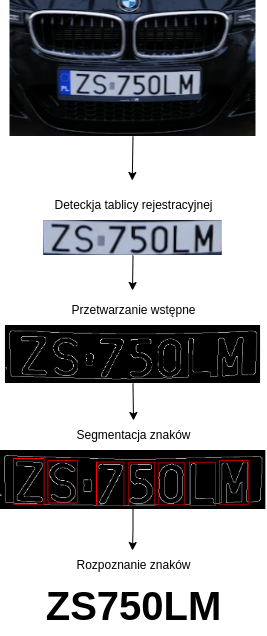
\includegraphics[scale=0.6]{Pictures/schemat_lpr}
    \caption{Etapy procesu automatycznego rozpoznawania tablic rejestracyjnych (źródło: opracowanie własne).}
    \label{fig:schemat_lpr}
\end{figure}
\FloatBarrier
Kolejne etapy korzystają z wyników uzyskanych w poprzednich krokach, co oznacza, że błąd powstały we wcześniejszej fazie, będzie rzutował na jakość działania całego systemu.
W wielu systemach zanim dojdzie do rozpoznawania tablicy rejestracyjnej, obraz jest w pierwszej kolejności odpowiednio przetwarzany.
Powszechnie stosowanymi czynnościami są: skalowanie obrazu, modyfikacje jasności oraz redukcja zakłóceń.
W zależności od wymagań stawianych przed danym mechanizmem i środowiskiem jego działania, czynności te mogą znacznie się od siebie różnić.
Najbardziej podstawowe systemy wymagają, aby pojazd znajdował się nieruchomo w określonym miejscu.
Tego typu rozwiązania najczęściej stosowane są na parkingach, gdzie szlaban otwiera się po odczycie numerów rejestracyjnych pojazdu i potwierdzeniu opłaty za postój w zewnętrznej bazie danych.
Takie systemy pracują z reguły w środowisku o niskim poziomie zakłóceń wynikających z warunków atmosferycznych i oświetlenia.
Obecnie na rynku znajduje się wiele komercyjnych rozwiązań, które oferują wysoką dokładność (powyżej 95\%) dla tego rodzaju detekcji.
Taki rodzaj systemów ARTR nazywany systemami statycznymi.
Dużo większą złożonością charakteryzują się systemy dynamiczne, w których znacznie większą rolę odgrywają zakłócenia wynikające ze zmiennych warunków oświetlenia.
W obecnych czasach stworzenie dynamicznego systemu ARTR o wysokiej dokładności wciąż stanowi wyzwanie i jest tematem wielu prac naukowych.
Celem niniejszej pracy jest analizowanie obrazów pochodzących z kamery samochodowej, co zdecydowanie sprawia, że jest to system dynamiczny.
Poniżej przedstawiono najczęściej stosowane metody widzenia komputerowego w systemach ARTR\@.


\section{Przegląd istniejących metod detekcji tablic rejestracyjnych}
\index{Przegląd istniejących metod detekcji tablic rejestracyjnych}

Zgodnie ze słowikiem języka polskiego, definicja tablicy rejestracyjnej brzmi następująco:
\begin{definition}[Tablica rejestracyjna]
    Płytka zawierająca numery identyfikacyjne pojazdu, umieszczana z przodu i z tyłu pojazdu.
\end{definition}
Dla programu komputerowego powyższe zdanie jest niezrozumiałe.
W zadaniu detekcji tablicy rejestracyjnej, wymagane jest, aby maszyna ,,zrozumiała'' jakich obiektów należy szukać.
W tym kontekście, za definicję można uznać ,,prostokątny obszar, z dużym zagęszczeniem horyzontalnych i wertykalnych krawędzi''~\cite{824138}.
W oparciu o powyższe cechy zaprezentowano wiele algorytmów do rozwiązania zadania wykrywania tablic rejestracyjnych.
Część z nich wywodzi się z tradycyjnych metod widzenia komputerowego i metod głębokiego uczenia.
Każda z metod ma swoje zalety, ale również często ograniczenia.
W związku z tym, trudno jednoznacznie stwierdzić, która z metod jest najbardziej efektywna.

Detekcja numerów rejestracyjnych jest wyzywającym zadaniem ze względu na poniższe czynniki:
\begin{itemize}
    \item zajmowanie niewielkiego obszaru na zdjęciu przez tablicę rejestracyjną,
    \item istnienie ogromnej ilości formatów tablic rejestracyjnych (w zależności od kraju rejestracji lub rodzaju pojazdu),
    \item słabe oświetlenie, rozmazany obraz, refleksy świetlne,
    \item ruch pojazdu, zabrudzone tablice.
\end{itemize}
Tradycyjne metody widzenia komputerowego oparte są na cechach takich jak kształt, kolor, symetria, tekstury itp.\cite{9310202}.
W celu uzyskania lepszych wyników, spotyka się rozwiązania, w których łączy się wiele technik.
Poniżej wyróżniono najczęściej stosowane metody w detekcji tablic rejestracyjnych.

\subsection{Metody oparte na krawędziach (ang. \textit{edge based)}}
\label{subsec:edge-based}
W większości krajów tablice rejestracyjne posiadają prostokątny kształt.
Dla poprawienia widoczności numerów pojazdów, stosuje się kolory o wysokim kontraście dla czcionki i tła.
Dzięki temu, tablice rejestracyjne zawierają wiele równoległych i prostopadłych linii.
Z uwagi na to, znaczna część badań bazuje na podejściu opartym o wykrywanie krawędzi.
W większości przypadków kolor tablicy rejestracyjnej jest różny od koloru pojazdu.
Dzięki temu, granice tablicy zostają uznane za krawędzie.
Wiele metod wykorzystuje filtr Sobela.
Jego działania polega na dyskretnym różniczkowaniu i aproksymacji pochodnych kierunkowych intensywności obrazu.
Filtr ten składa się z dwóch macierzy o wymiarach $3\times3$~\eqref{eq:sobel_matrices} służących do detekcji krawędzi horyzontalnych i wertykalnych.
\begin{equation}
    \begin{bmatrix}
        -1 & 0 & +1 \\
        -2 & 0 & +2 \\
        -1 & 0 & +1
    \end{bmatrix}
%
    \begin{bmatrix}
        +1 & +2 & +1 \\
        0  & 0  & 0  \\
        -1 & -2 & -1
    \end{bmatrix}
    \label{eq:sobel_matrices}
\end{equation}
Zaletą takiego podejścia jest niewątpliwa łatwość użycia, natomiast jedną z głównych wad jest jego wrażliwość na szum.

Często wykorzystywaną metodą do wykrywania krawędzi obiektów w obrazach jest \textit{Binary Image Processing}~\cite{4310039}.
Technika ta polega na sprowadzenia obrazu do postaci, w której kolory pikseli przyjmują tylko dwie wartości - czarną lub białą.
Osiąga się to za pomocą ustalenia progu, który determinuje kolor piksela.
Próg wyznaczany jest na podstawie histogramu obrazu w odcieniach szarości.
Metoda ta jest użyteczna, ze względu na fakt łatwego odseparowania obiektu od tła.
Wykorzystuje ona założenie, że krawędzie tablicy są proste i poziome.
Przy zdeformowanych lub zabrudzonych tablicach, algorytm ten nie osiąga zadowalających wyników.

Inną stosowaną metodą do wykrywania linii na obrazach binarnych jest transformata Hougha~\cite{DuanBuildingAA}.
Motywacją do jej opracowania była metoda siłowa (ang. \textit{brute force}), która jest jednak znacznie bardziej zasobożerna.
Złożoność algorytmu siłowego wynosi $O(n^3)$, gdzie $n$ oznacza liczbę niezbędnych operacji do wykonania.
Transformata Hougha polega na twierdzeniu, że każda prosta może być jednoznacznie przedstawiona za pomocą dwóch parametrów.
Przestrzeń tych parametrów to właśnie przestrzeń Hougha.
Najczęściej używanymi parametrami są współczynniki $\rho$ i $\alpha$ z równania prostej w postaci normalnej~\eqref{eq:transform_hough}
\begin{equation}
    \label{eq:transform_hough}
    x\cos{\alpha} + y\sin{\alpha} = \rho.
\end{equation}
W powyższym równaniu $\rho$ jest promieniem wodzącym, natomiast $\alpha$ kątem tworzonym przez $\rho$ z osią X.
W związku z powyższym, jest to algorytm o liniowej złożoności obliczeniowej.
Można wykazać następujące własności transformacji Hougha:\\
\begin{theorem}
    Prostej przestrzeni kartezjańskiej odpowiada w przestrzeni Hougha punkt, natomiast
    punktowi przestrzeni kartezjańskiej odpowiada w przestrzeni Hougha sinusoidalna krzywa.
    Punkty leżące na tej samej prostej korespondują z sinusoidami przechodzącymi przez
    wspólny punkt w przestrzeni Hougha~\cite{hough_transform_definition}.
\end{theorem}
Zasadę transformacji ilustruje Rysunek~\ref{fig:hough_transform}.
\begin{figure}[!ht]
    \centering
    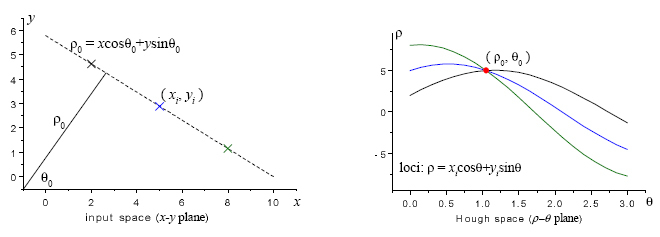
\includegraphics[scale=1]{Pictures/hough_transform.jpeg}
    \caption{Transformata Hougha (źródło:~\cite{Lin:01}).}
    \label{fig:hough_transform}
\end{figure}
\FloatBarrier

Innym spotykanym podejściem~\cite{4410602} jest stosowanie dwóch algorytmów.
Pierwszy z nich ma za zadanie wyodrębnić odcinki linii i pogrupować je na podstawie wcześniej ustalonego zbioru warunków geometrycznych.
Drugi znajduje obszary o najwyższym zagęszczeniu pionowych krawędzi.
Dzięki takiemu spojrzeniu na przedstawiony problem, uzyskane wyniki mają wysoką dokładności, szczególnie dla pojazdów znajdujących się w ruchu.
Metode oparte na krawędziach są stosowane w wielu rozwiązaniach ze względu na ich szybkość działania i prostotę.
Jednakże, rozwiązania te są silnie wrażliwe na niepożądane krawędzie i nie sprawdzają się w rozmytych i złożonych obrazach.

\subsection{Metody oparte na kolorach (ang. \textit{color based)}}
\label{subsec:color-based}
Metody oparte na kolorach bazują na fakcie, że kolor tablicy jest różny od koloru tła pojazdu.
Dla tej grupy rozwiązań, zamiast modelu barw RGB, stosuje się model HSL oparty o nasycenie koloru.
Model ten jest jednak wrażliwy na szum.

Często metody wykorzystujące kolor tablicy rejestracyjnej są używane do wyselekcjonowania kandydatów.
Innymi słowy, oznacza to wybrania obszarów obrazu, w których może znajdować się tablica rejestracyjna.
Technika ta łączona jest z innymi algorytmami, które na kolejnych etapach decydują, czy wskazany obszar rzeczywiście zawiera poszukiwany obiekt.
Do tego typu metod wykorzystywany jest m.\ in.\ algorytm \textit{Mean shift}~\cite{1520110} i logika rozmyta~\cite{Wang2008FuzzybasedAF}.

Opisywana grupa metod może zostać użyta do detekcji zdeformowanych i pochylonych tablic.
Rzadko występują one osobno w metodach detekcji, głównie ze względu na ich dużą czułość na zmiany naświetlenia.
Dodatkowo w zależności od kraju oraz przeznaczenia pojazdu, kolory tablic mogą się znacznie różnić.
Przykładowo obecnie w Polsce tablice aut elektrycznych mają kolor zielony, a samochodów zabytkowych żółty, patrz Rys.~\ref{fig:tablice}.
\FloatBarrier
\begin{figure}[!ht]
    \centering
    
\includegraphics[scale=0.6]{Pictures/tablice}
    \caption{Tablice rejestracyjne w Polsce dla aut elektrycznych i zabytkowych (źródło: opracowanie własne).}
    \label{fig:tablice}
\end{figure}
\FloatBarrier

\subsection{Metody oparte na teksturach (ang. \textit{texture based)}}
\label{subsec:metody-oparte-na-teksturach}
Metody oparte na teksturach wykorzystują fakt znajdowania się znaków na tablicach rejestracyjnych.
Znaki na tablicy mają z reguły czarny kolor i znajdują się na jasnym tle tworząc duży kontrast.
Powyższa grupa algorytmów wykorzystuje wysoką częstość zmiany kolorów w obszarze występowania tablic rejestracyjnych.
W~\cite{824138} autorzy zaproponowali metodę lokalizacji tablic wykorzystując algorytm kwantowania wektorowego (ang. \textit{Vector Quantization - VQ}).
W przeciwieństwie do innych metod, które wykorzystywały krawędzie lub kontrast, metoda VQ wykorzystuje aktualną zawartość tablicy rejestracyjnej.
Autorzy wykazali bardzo wysoką skuteczność rozwiązania na poziomie 98\%.

W analizie tekstur, często stosuje się filtr Gabora.
Jest to filtr liniowy, pozwalający na przefiltrowanie obrazu z precyzyjnie dobranym zakresem częstotliwości.
Reprezentacje częstotliwości i orientacji filtrów Gabora są uważane przez wielu współczesnych naukowców zajmujących się widzeniem komputerowym za podobne do tych z ludzkiego układu wzrokowego~\cite{gabor_human_eye}.
W~\cite{gabor_lpr} zaprezentowano algorytm wykorzystujący filtr Gabora.
Jest to jednak metoda czasochłonna i nie znajduje zastosowania w systemach, w których szybkość działania jest jednym z najistotniejszych czynników.

Wszystkie metody oparte na teksturach są odporne na deformacje tablic.
Jest to kluczowa zaleta ich stosowania.
Mimo to, metody te wymagają skomplikowanych obliczeń i nie dają zadowalających efektów w złożonych środowiskach z różnymi warunkami oświetlenia.

\subsection{Klasyfikatory}\label{subsec:klasyfikatory}
Wiele badań wykorzystuje cechy Haara razem z algorytmem AdaBoost (ang. \textit{Adaptative Boosting --- AdaBoost}) do wyuczenia kaskady klasyfikatorów~\cite{9310202}.
Podejście takie zostało zaproponowane po raz pierwszy w~\cite{990517}.
Algorytm Violi-Jonesa został zaprezentowany w 2001.
Wykorzystuje on algorytm AdaBoost, który został zaproponowany w pracy~\cite{Freund1996ExperimentsWA}.
Pomimo upływu ponad 20 lat, dalej jest on powszechnie stosowany, co świadczy o jego ponadczasowości i uniwersalności.
Autorzy zaprojektowali go jako detektor twarzy, jednak jego funkcjonalność pozwala na wykrywanie dowolnych obiektów, np\. tablic rejestracyjnych, przy odpowiednim wyuczeniu.
Aby przedstawić, jak działa algorytm Violi-Jonesa, należy najpierw zrozumieć czym są cechy Haara.

Cechy Haara często są przedstawiane jako skalowalne, prostokątne szablony (Rysunek~\ref{fig:haar_feats}), używane do porównania zależności pomiędzy pikselami.
Reprezentują one zgrubne kontury obiektu.
Obraz skanowany jest oknem przesuwnym o rozmiarze zbliżonym do poszukiwanego obiektu.
Dla każdego okna obliczane są wartości cech Haara, na podstawie, których klasyfikator podejmuje decyzję.
Wartość pojedynczej cechy obliczana jest jako różnica pomiędzy średnią jasnością pikseli w zbiorze ,,białym'' i średnią jasnością pikseli w zbiorze ,,czarnym''~\cite{szybka_detekcja_klesk}.
\begin{figure}[!ht]
    \centering
    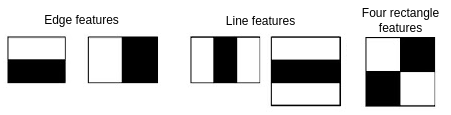
\includegraphics[scale=0.6]{Pictures/haar_feats}
    \caption{Cechy Haara używane w algorytmie Violi-Jonesa (źródło: \url{https://docs.opencv.org/4.x/d2/d99/tutorial_js_face_detection.html}).}
    \label{fig:haar_feats}
\end{figure}
\FloatBarrier
Im większa będzie liczba okien w procedurze skanującej, tym większa będzie niezbędna liczba cech do wyliczenia.
Zauważono, że cechy mogą być jednak wyznaczane w czasie stałym, niezależnym od rozmiaru okna.
W tym celu należy przygotować przed procedurą detekcji dodatkową tablicę zwaną obrazem całkowym (ang. \textit{integral image}).
Obrazem całkowym nazywamy tablicę dwuwymiarową o rozmiarze obrazu źródłowego, w której każdy element w i-tym wierszu i j-tej kolumnie przechowuje sumę pikseli z tej części obrazu, której prawym dolnym wierzchołkiem jest piksel $(i, j)$.
%\begin{figure}[!htb]
%    \centering
%    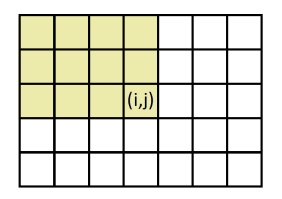
\includegraphics[scale=0.6]{Pictures/ii_cords}
%    \caption{Obraz całkowy dla punktu $(i, j)$ (źródło: \url{https://www.spoj.com/WIPING5/problems/WIPING50.pdf}).}
%    \label{fig:ii_cords}
%\end{figure}
%\FloatBarrier
Matematycznie obraz całkowy $ii(x,y)$ przedstawiamy jako:
\begin{equation}
    \label{eq:integral_image}
    ii(x,y) = \sum_{1\leq j \leq x} \sum_{1\leq k \leq y} i(j,k).
\end{equation}
%czym innym jest obliczanie sumy a czym inne szybkie obliczanie obrazu całkowego
Obliczanie obrazu całkowego z definicji~\eqref{eq:integral_image} dla każdego punktu w obrazie jest czasochłonne i charakteryzuje się złożonością obliczeniową $O(n_x^2 n_y^2)$.
Sposobem na szybsze obliczenie obrazu całkowego może być wykorzystanie wzorów rekurencyjnych~\cite{990517,10.1145/800031.808600}:
\begin{equation}
    \label{eq:integral_image_induction}
    s(j,k)=s(j, k-1)+f(j,k),
\end{equation}
\begin{equation}
    \label{eq:integral_image_induction2}
    ii(j,k)=ii(j,k-1)+s(j,k),
\end{equation}
gdzie $s(j,k)$ to skumulowana suma w wierszu, $f(j,k)$ to wartość obrazu w punkcie $(j,k)$~\cite{990517}.
Dzięki takiemu rozwiązaniu, wyznaczanie obrazu całkowego charakteryzuje się złożonością obliczeniową $O(n_x n_y)$.

Kiedy obraz całkowy został wyznaczony, obliczenie sumy jasności dla dowolnego fragmentu obrazu jest operacją o stałej złożoności obliczeniowej $O(1)$.
Aby osiągnąć złożoność niezależną od rozmiaru okna, sumę oblicza się odejmując od sumy wartości obrazu całkowego dla prawego dolnego i lewego górnego wierzchołka sumę wartości obrazu dla pozostałych wierzchołków analizowanego prostokąta.
Poniżej przedstawiono obliczenie sumy dla prostokąta rozpiętego między punktami $(x_1, y_1)$, a $(x_2, y_2)$.
\begin{equation}
    \label{eq:integral_image_x_y}
    \sum_{x_1\leq x \leq x_2} \sum_{y_1\leq y \leq y_2} i(x,y) = ii(x_2, y_2) - ii(x_1 - 1, y_2) - ii(x_2, y_1 - 1) + ii(x_1 - 1, y_1 - 1)
\end{equation}
Na podstawie powyższego wzoru można zauważyć, że wystarczą operacje tylko na 4 punktach obrazu całkowego~\cite{szybka_detekcja_klesk}.
Dla obliczenia różnicy pomiędzy sumami dwóch dowolnych prostokątów wymagane jest pobranie wartości dla 8 punktów z obrazu całkowego.
Poprzez zastosowanie skalowania szablonów i zakotwiczanie ich w różnych miejscach badanego okna, możliwe jest uzyskanie dużej (tzn.\ rzędu $10^3$ lub $10^4$) ilości cech Haara bez konieczności skalowania obrazu.
Tak duża liczba cech wymagana jest na etapie uczenia klasyfikatora.
Dzięki zastosowaniu boostingu, algorytm dokonuje selekcji znacznie mniejszej liczby cech, które zapewnią dobry opis rozpatrywanych obiektów w danym zagadnieniu detekcji.

%TODO - przenieść to dalej, a tutaj dać o boostingu
%Algorytm Violi-Jonesa wymaga dużej ilości próbek pozytywnych i negatywnych.
%Do wyuczenia klasyfikatora i wybrania zbioru cech zastosowano algorytm AdaBoost.
%Autorzy zaproponowali użycie kaskady klasyfikatorów.
%Takie podejście bazuje na obserwacji, że okna pozytywne stanowią średnio $0.01\%$ wszystkich okien.
%Rozpatrywane okno w pierwszej kolejności badane jest przez słabsze klasyfikatory, które bazują na mniejszej liczbie cech.
%Dzięki takiemu podejściu algorytm stał się bardziej wydajny czasowo.
%Każdy kolejny klasyfikator w kaskadzie oblicza większą liczbę cech.
%Jeżeli na którymś etapie klasyfikator zwróci odpowiedź negatywną, proces jest przerywany.
%Do osiągnięcia pozytywnego wyniku, wymagane jest zwrócenie przez wszystkie klasyfikatory odpowiedzi pozytywnej.
%W algorytmie Violi-Jonesa kaskada składa się z 32 klasyfikatorów, które badają od 2 do 200 cech.
%Łącznie liczone jest 4297 cech, co daje średnio 8 cech na klasyfikator.
%W trakcie uczenia każdy z klasyfikatorów ma przypisany indywidualny próg decyzyjny.
%Każdy etap kaskady uczony jest w ramach boostingu (np. poprzez AdaBoost lub RealBoost).

AdaBoost (Adaptive Boosting) to algorytm, którego zadaniem jest stworzenie mocnego klasyfikatora na podstawie wielu słabych klasyfikatorów.
Słabym klasyfikatorem nazywamy klasyfikator, który osiąga niską dokładność, jednak wyższą od losowych wyników.
Za przykład może posłużyć rozpoznawanie płci na podstawie wzrostu.
Słaby klasyfikator mógłby bazować na założeniu, że każda osoba o wzroście 175cm lub wyższym jest mężczyzną.
Pozostała grupa osób jest kobietami.
Wiele osób ze zbioru testowego zostanie określonych błędnie, jednak dokładność klasyfikatora będzie wyższa niż 50\%.
AdaBoost jest techniką, która może zostać łączona z dowolnym algorytmem klasyfikującym, jednak nie może zostać wykorzystany jako samodzielny klasyfikator.
Po raz pierwszy został on przedstawiony w~\cite{Freund1996ExperimentsWA}.
AdaBoost występuję w połączeniu z popularnymi wariantami słabych klasyfikatorów~\cite{szybka_detekcja_klesk}:
\begin{itemize}
    \item AdaBoost + decision stump
    \item AdaBoost + drzewka decyzyjne
    \item AdaBoost + klasyfikator liniowy (np. SVM)
    \item AdaBoost + naiwny Bayes
\end{itemize}
Głównymi zastosowaniami tej techniki jest wybór najlepszych cech z punktu widzenia klasyfikacji oraz dobór wag dla klasyfikatorów wchodzących w skład kaskady.


Tutaj dać pseudokod algorytmu i następnie go opisać\\
%\begin{algorithmic}
%    \If {$i\geq maxval$}
%        \State $i\gets 0$
%    \Else
%        \If {$i+k\leq maxval$}
%            \State $i\gets i+k$
%        \EndIf
%    \EndIf
%\end{algorithmic}

Każdy słaby klasyfikator uczony jest na tym samym podzbiorze.
Każda próbka ma przypisaną wagę, która mówi o jej istotności z punktu uczenia klasyfikatora.
Dla każdego kolejnego słabego klasyfikatora, próbki są reważone w ten sposób, aby błędnie sklasyfikowane próbki
AdaBoost przypisuje wagi do jednostek treningowych, które określają prawdopodobieństwo pojawienia się w zbiorze uczącym zgodnie ze wzorem~\eqref{eq:treaning_unit_weight_adaboost}.
\begin{equation}
    \label{eq:treaning_unit_weight_adaboost}
    D_{t+1}(i) = \dfrac{D_t(i) \exp(-\alpha_t y_i h_t(x_i))}{Z_t}
\end{equation}
$D_t$ oznaczono wektor wszystkich wag, natomiast $Z_t$ reprezentuje ich sumę.
Indeks $i$ jest numerem kolejnej próbki w zbiorze uczącym.
Na początku wszystkie próbki posiadają tą sama wartość wag.
Po zakończeniu uczenia, wagi błędnie sklasyfikowanych próbek zostają zwiększone.
Dzięki temu, w następnej iteracji uczenia kolejny klasyfikator będzie mógł lepiej rozpoznawać niepoprawnie oznaczone jednostki treningowe w poprzednim kroku.
W momencie, gdy każdy klasyfikator zostanie wyuczony, AdaBoost przypisuje do nich wagi na podstawie dokładności każdego z nich.
Ostateczną odpowiedź klasyfikatora można opisać wzorem~\eqref{eq:ada_boost_clf}.
\begin{equation}
    \label{eq:ada_boost_clf}
    H(x) = \sign\left(\sum_{t=1}^{T} \alpha_t h_t(x))\right)
\end{equation}
Finalny klasyfikator zawiera $T$ słabych klasyfikatorów.
Waga klasyfikatora, wyliczona przez AdaBoost, została określona symbolem $\alpha_t$.
Ostateczny rezultat powyższego równania można opisać jako liniowa kombinacja słabych klasyfikatorów.

Pierwszy klasyfikator ($t=1$) jest trenowany z równym prawdopodobieństwem dla wszystkich próbek.
Po zakończeniu uczenia, waga obliczana jest na podstawie wzoru~\eqref{eq:weight_clf}.
\begin{equation}
    \label{eq:weight_clf}
    \alpha_t = \dfrac{1}{2} \ln \dfrac{1-\epsilon_t}{\epsilon_t}
\end{equation}
Współczynnik $\alpha_t$ jest skorelowany z poziomem błędu klasyfikatora $\epsilon_t$, który to jest liczony jako liczba błędnie sklasyfikowanych próbek dzielona przez rozmiar zbioru uczącego.
Rysunek~\ref{fig:adaboost_alphacurve} przedstawia powyższą zależność.
\begin{figure}[!ht]
    \centering
    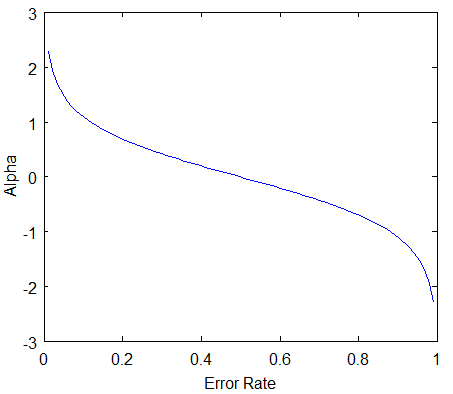
\includegraphics[scale=0.6]{Pictures/adaboost_alphacurve}
    \caption{Zależność współczynnika $\alpha$ od błędu klasyfikatora (źródło: \url{https://chrisjmccormick.files.wordpress.com/2013/12/adaboost_alphacurve.png}).}
    \label{fig:adaboost_alphacurve}
\end{figure}
\FloatBarrier
Z Rysunku~\ref{fig:adaboost_alphacurve} można odczytać, że waga rośnie wykładniczo dla klasyfikatorów o wysokiej dokładności.
Dla klasyfikatora o poziomie błędu 0.5 waga jest równa zero.
Oznacza to, że taki klasyfikator jest równie dokładny co losowe zgadywanie, dlatego jest on ignorowany.
Dla klasyfikatorów o większym poziomie błędu, waga przyjmuje wartość ujemną.
Jeśli taki klasyfikator uzna próbkę za negatywną, ostatecznie zostanie ona oznaczona jako pozytywna.

AdaBoost jest techniką uczenia progresywnego.
Ważne jest, aby na wejściu próbki uczące były odpowiedniej jakości.
Metoda ta jest bardzo czuła na zakłócenia.
Jednymi z najczęstszych aplikacji tego typu boostingu jest klasyfikacja tekstu oraz zdjęć.

Wzmocnienie AdaBoost spotykane jest w różnych wariantach.
Jednym z nich jest Real AdaBoost, zwany również RealBoostem, zaprezentowany po raz pierwszy w~\cite{10.1023/A:1007614523901}.
Główną różnicą w stosunku do AdaBoosta, jest założenie, że słabe klasyfikatory są rzeczywistoliczbowe, a nie binarne~\cite{szybka_detekcja_klesk}.
Odpowiedź słabego klasyfikatora jest zwykle ustalana jako przybliżenie połowy przekształcenia logit:
\begin{equation}
    \label{eq:real_boost}
    f_t(X) =\dfrac{1}{2}\ln\dfrac{\hat{P_w}(y=1|x)}{\hat{P_w}(y=-1|x)}
\end{equation}
gdzie $\hat{P_w}(y=\pm1|x)$ stanowi oszacowanie rozkładu klas warunkowego na $x$ z wykorzystaniem aktualnych wag $w_i$.
W przeciwieństwie do AdaBoost, słabe klasyfikatory nie posiadają wag.
Mechanizm ważenia słabych klasyfikator jest niejako wpleciony w same odpowiedzi rzeczywistoliczbowe.
Możliwym jest wykazanie, że wyrażenie~\eqref{eq:real_boost} jest rozwiązaniem zadania minimalizacji kryterium wykładniczego określonego poprzez rozkład ${w_i}$ na zbiorze danych (tj.\ na konkretnej próbie).
Analogicznie wyrażenie to jest również rozwiązaniem zadania minimalizacji kryterium wykładniczego określonego poprzez prawdziwy ale nieznany rozkład łączny generujący dane tj. $P(x,y)=p(x)P(y|x)$~\cite{szybka_detekcja_klesk}.
Algorytm RealBoost posiada silne podobieństwa do techniki regresji logistycznej.
Schemat reważenia w boostingu pracuje sposób pokrewny do rezyduów błędów (ang. \textit{error residuals}).

%TODO - poprawka koszyków
Jednym ze słabych klasyfikatorów stosowanych razem z algorytmem RealBoost są tzw.\ koszyki (ang. \textit{response binning}).
Ten typ klasyfikatora został zaprezentowany w~\cite{1689652}.
Przedstawiony sposób działania polega na przybliżaniu rozkładów warunkowych przez funkcje kawałkami stałe~\cite{szybka_detekcja_klesk}.
Przed uczeniem algorytmu wyznacza na jest liczba koszyków o równej szerokości oznaczana literą $B$.
Na podstawie ustalonych przedziałów $[a_1,a_2]$, każdej z cech przypisywany jest odpowiedni indeks koszyka.
Indeks koszyka $\beta(x) \in \{1,\dots,B\}$, do którego należy $x$ obliczany jest na podstawie wzoru~\eqref{eq:bin_index}.
\begin{equation}
    \label{eq:bin_index}
    \beta(x)=\left.
    \begin{cases}
        B(x - a_1)/(a_2-a_1), & \text{dla } a_1 \leq x \leq a_2 \\
        1, & \text{dla } x \leq a_1 \\
        B, & \text{dla } a_2 < x
    \end{cases}
    \right.
\end{equation}
Odpowiedź słabego klasyfikatora dla $j^*$-tej cechy przedstawia wzór~\eqref{eq:bin_weak_clf}, gdzie $\hat{P_w}(y=-1, j\;jest\;w\;b)=\sum_{\{i:y_i=-1,\beta(x_ij)=b\}}^{} w_i$ oznacza szacowane prawdopodobieństwo zdarzenia, że przykład jest negatywny a jego $j$-ta cecha należy do kosza $b$.
\begin{equation}
    \label{eq:bin_weak_clf}
    f_t(x;j^*) = \dfrac{1}{2} \ln\dfrac{\hat{P_w}(y=1, j^*\;jest\;w\;\beta(x_j^*))}{\hat{P_w}(y=-1, j^*\;jest\;w\;\beta(x_j^*))}
\end{equation}
Autorzy algorytmu zalecają stosowanie dużej ilości koszyków dla gładkiego histogramu rozkładu cech.
Jeżeli histogram zawiera wiele maksimum lokalnych, należy zmniejszyć liczbę koszyków.
W przeciwnym razie zbyt duża rozdzielczość może wprowadzić szum do klasyfikatora, natomiast zbyt niska liczba koszyków może pozbawić klasyfikatora istotnych cech~\cite{1689652}.

\subsection{Metody głębokiego uczenia (ang. \textit{Deep learning})}
W związku z rozwojem dziedziny widzenia komputerowego oraz wzrostem mocy komputerów na przestrzeni ostatnich lat, wiele metod statystycznych zostało zastąpionych przez sieci neuronowe z powodu ich wysokiej skuteczności w detekcji obiektów.
Jednym z zaproponowanych podejść jest użycie sieci konwolucyjnych (ang. \textit{Convolutional Neural Network} --- CNN)\cite{cnn_detector}.
Składają się one z jednej lub wielu warstw konwolucyjnych (typowych dla kroku próbkowania, określającego subwzorce), a następnie przez jedną lub w pełni połączone warstwy tak jak w klasycznej wielowarstwowej sieci, np. MLP,SVM, SoftMax itp.
Sieci kowolucyjne są łatwe do uczenia, gdyż zawierają mniej parametrów (wykorzystując te same wagi) niż typowe sieci neuronowe z dokładnością do ilości warstw konwolucyjnych i ich rozmiaru.
Ten rodzaj sieci neuronowych jest predestynowany do obliczeń na strukturach 2D (tj\. obrazy)~\cite{cnn_agh}.

Jednym z najnowocześniejszych systemów detekcji w czasie rzeczywistych jest algorytm YOLO (ang. \textit{You only look once})~\cite{7780460}.
Algorytm jest bardzo wydajny.
Bazuje na sieciach R-CNN.
Autorzy zapewniają o możliwości przetwarzania 45 klatek na sekundę, a dla wersji szybszej, lecz o niższej dokładności, ponad 150 klatek na sekundę.
Twórcom wzorca przyświecała idea ,,spojrzenia tylko raz'', wzorując się na postrzeganiu świata przez człowieka, który po jednym spojrzeniu na badany obraz, jest w stanie zidentyfikować konkretne obiekty.
W przeciwieństwie do tradycyjnych metod z oknem przesuwnym, YOLO podczas procesu uczenia i testowania otrzymuje na wejściu cały obraz.
Na obraz wejściowy nałożona zostaje siatka o rozmiarze SxS, która tworzy obwiednie, a następnie wykorzystuje je do rozpoznawania szukanych obiektów.
Dla każdej uzyskanej ramki, mechanizm wyznacza prawdopodobną klasę.
Ramki o prawdopodobieństwie wyższym od ustalonego progu, zostają nałożone na wejściowy obraz, najczęściej w postaci prostokątów otaczających obiekt.
Rysunek~\ref{fig:yolo} przedstawia opisany schemat.
Ograniczenia YOLO wynikają z ograniczeń przestrzennych algorytmu.
W zależności od wielkości siatki, system może mieć problem z wykryciem mniejszych obiektów takich jak np. stado ptaków.
Algorytm jest stale udoskonalany przez autorów.
Na moment pisania pracy, udostępniona została trzecia wersja systemu.
\begin{figure}[!ht]
    \centering
    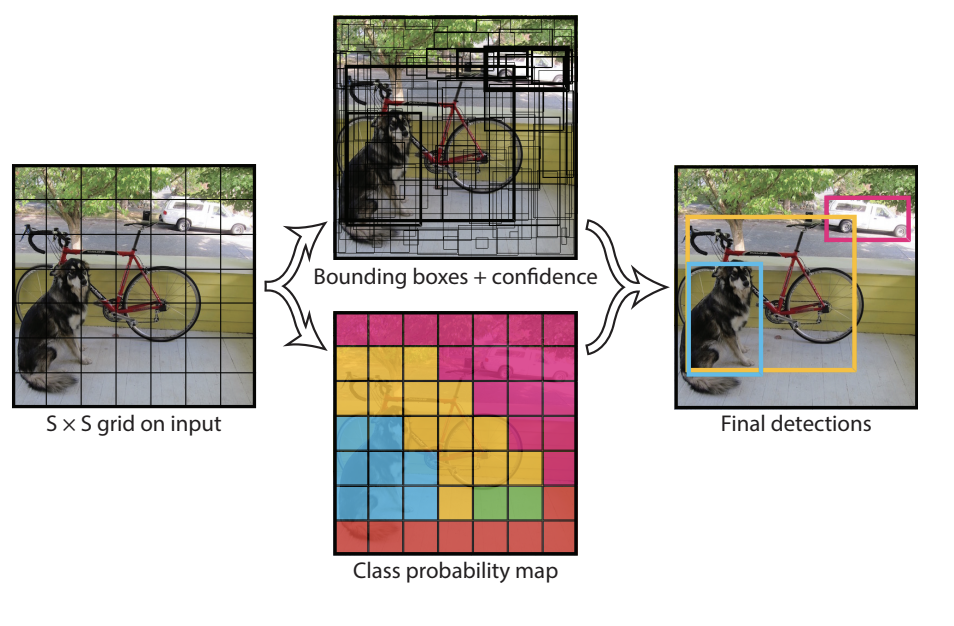
\includegraphics[scale=0.4]{Pictures/yolo}
    \caption{Algorytm YOLO (źródło: \url{https://towardsdatascience.com/r-cnn-fast-r-cnn-faster-r-cnn-yolo-object-detection-algorithms-36d53571365e}).}
    \label{fig:yolo}
\end{figure}
\FloatBarrier


\section{Przegląd istniejących metod segmentacji tablic rejestracyjnych}
\index{Przegląd istniejących metod segmentacji tablic rejestracyjnych}

Drugim etapem w większości systemów Automatycznego Rozpoznawania Tablic Rejestracyjnych jest rozpoznanie znaków na tablicy rejestracyjnej zlokalizowanej w poprzednim kroku.
Zanim dojdzie do klasyfikacji znaków, często są one wpierw segmentowane.
Jest to szczególny przypadek optycznego rozpoznawania znaków~\cite{9310202}.
Wiele krajów posiada ścisłe regulacje na temat czcionki i kolorów tablicy rejestracyjnej.
Przepisy te mają na celu zwiększenie czytelności znaków identyfikujących każdy pojazd.
W Polsce, jak i większości krajów na świecie, tablice pokryte są specjalną warstwą refleksyjną odbijającą światło.
Działanie takie zwiększa ich czytelność dla ludzkiego oka w gorszych warunkach oświetleniowych.
Dla aparatów fotograficznych ta cecha tablic często powoduje nieczytelność tablic na wykonanym zdjęciu.
Tablica odbija na tyle dużą ilość światła, co skutkuje powstaniem na zdjęciu białego prostokąta w miejscu tablicy.
Przykład takiego obrazu przedstawia Rysunek~\ref{fig:refleks_swietlny}.
\begin{figure}[!ht]
    \centering
    \includegraphics[scale=0.8]{Pictures/refleks_świetlny}
    \caption{Refleks świetlny występujący w niewystarczających warunkach oświetleniowych (źródło: opracowanie własne).}
    \label{fig:refleks_swietlny}
\end{figure}
\FloatBarrier
Poza powyższymi trudnościami, tablice mogą być obrócone lub uszkodzone.
Aby zwiększyć w jak największym stopniu prawdopodobieństwo prawidłowego odczytania znaków, używa się szereg czynności na obrazie wejściowym.
Dla obróconych obiektów stosuje się transformatę biliniową, zwaną również metodą Tustina~\cite{Xu2006AMO}.

\subsection{Binaryzacja}\label{subsec:binaryzacja}
W wielu klasycznych metodach widzenia komputerowego, w celu segmentacji znaków, stosuje się binaryzację.
W zbinaryzowanym obrazie łatwiej jest rozdzielić znaki w porównaniu do obrazu kolorowego lub w skali szarości.
Podstawowym problemem tej techniki jest odpowiedni dobór wartości progu.
Wybór ten jest dokonywany w oparciu o różne metody, które można podzielić na zmiennoprogowe i automatyczne.
Jednakże, wyznaczenie progu binaryzacji musi zostać wykonane właściwie, w celu uniknięcia połączenia znaków lub scalenia ich z obramowaniem tablicy rejestracyjnej~\cite{6213519}.
Jednym z częściej stosowanych metod binaryzacji jest progowanie adaptacyjne (ang. \textit{Adaptive Thresholding}).
Stosuje się to w momencie kiedy różne obszary obrazu mogą charakteryzować się różnymi warunkami oświetlenia i stosowanie stałej wartości nie dałoby zadowalających efektów.
Algorytm wyznacza próg dla konkretnego piksela na podstawie niewielkiego regionu wokoło.
Dla tego samego obrazu wyliczane są różne wartości progu dla różnych regionów co prowadzi do uzyskania lepszych wyników niż w przypadku stałego progu binaryzacji.
Na Rysunku~\ref{fig:threshold} przedstawiono przykłady binaryzacji obrazu stałym progiem globalnym i progiem wyznaczonym adaptacyjnie.
\begin{figure}[!ht]
    \centering
    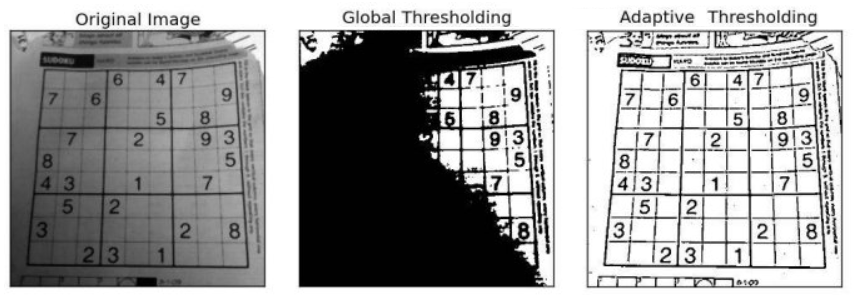
\includegraphics[scale=0.6]{Pictures/threshold}
    \caption{Przykład binaryzacji obrazu przy niejednorodnym oświetleniu za pomocą globalnego i lokalnego progu (źródło: \url{https://docs.opencv.org/3.4/d7/d4d/tutorial_py_thresholding.html}).}
    \label{fig:threshold}
\end{figure}
\FloatBarrier

Algorytm progowania adaptacyjnego otrzymuje najczęściej na wejściu obraz w skali szarości lub kolorowy.
Próg jest wyliczany dla wszystkich pikseli w obrazie z osobna.
Jednym ze znanych podejść jest to zaproponowane przez Chow i Kaneko~\cite{Chow1971BoundaryDO}.
W tym przypadku obraz dzielony jest na zbiór nakładających się fragmentów.
Optymalny próg wyznaczy jest dla konkretnego fragmentu na podstawie analizy histogramu.
Próg dla każdego piksela wyliczany jest na podstawie interpolacji wyników dla odpowiedniego fragmentu.
Wadą tej metody jest jej złożoność obliczeniowa.
Jest to jeden z głównych powodów, dlaczego algorytm ten nie znalazł zastosowania w aplikacjach działających w czasie rzeczywistym.

Alternatywnym podejściem do znalezienia lokalnego progu jest statystyczne zbadanie intensywności sąsiedztwa każdego piksela.
Wybór metody statystycznej jest skorelowany z obrazem wejściowym.
Najczęściej używa się średniej, mediany, średniej z wartości maksymalnej i minimalnej badanego otoczenia lub funkcji Gaussa.
Dobór wielkości sąsiedztwa ma duży wpływ na wyliczenie progu.
Rozmiar musi być na tyle duży, aby zawierać zarówno piksele tła jak i badanego obiektu.
Z drugiej strony wybranie zbyt dużych obszarów może naruszyć założenie o równomiernym oświetleniu rozpatrywanego fragmentu.
Ten rodzaj adaptycyjnego progowania jest bardziej wydajny od algorytmu Chow i Kaneko.
Charakteryzuje się wysoką jakością oddzielania obiektów od tła i znajduje szerokie zastosowanie w wielu aplikacjach.

Innym znanym algorytmem stosowanym do wyznaczania progu binaryzacji jest algorytm Otsu~\cite{4310076}.
Metoda Otsu jest techniką opartą na wariancji w celu znalezienia wartości progowej, przy której ważona wariancja między pikselami pierwszego planu i tła jest najmniejsza~\cite{otsu_article}.
Kluczową ideą jest tutaj iteracja przez wszystkie możliwe wartości progu i pomiar rozproszenia pikseli tła i pierwszego planu.
Następnie znajdowany jest próg, w którym rozproszenie jest najmniejsze.
Algorytm iteracyjnie wyszukuje próg, który minimalizuje wariancję wewnątrz klasy, zdefiniowaną jako ważona suma wariancji dwóch klas (tła i pierwszego planu).
Kolory w skali szarości zwykle mieszczą się w zakresie 0-255.
Tak więc, jeśli wybierzemy próg 100, to wszystkie piksele o wartościach mniejszych niż 100 staną się tłem, a wszystkie piksele o wartościach większych lub równych 100 staną się pierwszym planem obrazu.
Wzór na znalezienie wariancji wewnątrz klasowej przy dowolnym progu $t$ jest określony wzorem~\eqref{eq:otsu_variance}
\begin{equation}
    \label{eq:otsu_variance}
    \sigma^2(t)=\omega_{bg}(t)\sigma_{bg}^2(t)+\omega_{fg}(t)\sigma_{fg}^2(t)
\end{equation}
gdzie $\omega_{bg}(t)$ i $\omega_{fg}(t)$ reprezentują prawdopodobieństwo liczby pikseli dla każdej klasy przy progu $t$, natomiast $\sigma^2$ oznaczono wariancję wartości kolorów.
Wyliczanie wariancji dla konkretnej klasy pikseli przedstawiono na wzorze~\eqref{eq:otsu_variance_value}.
\begin{equation}
    \label{eq:otsu_variance_value}
    \sigma_{bg | fg}^2(t)=\dfrac{\sum_{}^{}(x_i-\hat{x})^2}{N-1}
\end{equation}
Wartość piksela odpowiedniej klasy reprezentuje symbol $x_i$, natomiast $\hat{x}$ reprezentuje średnią pikseli rozpatrywanej klasy.
Liczbę wszystkich pikseli zapisano literą $N$.

Metoda Otsu implementowana przez wiele środowisk obliczeniowych (np. MATLAB)~\cite{otsu_inzynieria_rolnicza}.
Algorytm szczególnie dobrze sprawdza się w przypadkach, gdy liczby pikseli tła i obiektów pierwszego planu są zbliżone~\cite{10.1117/1.1631315}.

\subsection{Metoda k-średnich (ang. \textit{ang. K-Means algorithm})}
todo~\cite{segmentation_kmeans}

\subsection{Metoda rzutów jasności}
todo

\subsection{Metoda elementów połączonych (ang. \textit{Connected components})}
todo


\section{Przegląd istniejących metod rozpoznawania tablic rejestracyjnych}
\index{Przegląd istniejących metod rozpoznawania tablic rejestracyjnych}

\subsection{OCR}
tesseract korzysta z sieci lstm wiec warto by to opisać i jakieś inne sieci
%https://bulldogjob.pl/readme/3-typy-rekurencyjnych-sieci-neuronowych

\subsection{Metody oparte na wzorcach}
@TODO - TEMPLATE AND PATTERN MATCHING TECHNIQUES % chapter1.tex zawiera treść rozdziału 1

%----------------------------------------------------------------------------------------
%	ROZDZIAŁ 2
%----------------------------------------------------------------------------------------
    %%%%%%%%%%%%%%%%%%%%%%%%%%%%%%%%%%%%%%%%%
% Szablon pracy dyplomowej
% Wydział Informatyki 
% Zachodniopomorski Uniwersytet Technologiczny w Szczecinie
% autor Joanna Kołodziejczyk (jkolodziejczyk@zut.edu.pl)
% Bardzo wczesnym pierwowzorem szablonu był
% The Legrand Orange Book
% Version 2.1 (26/09/2018)
%
% Modifications to LOB assigned by %JK
%%%%%%%%%%%%%%%%%%%%%%%%%%%%%%%%%%%%%%%%%


%----------------------------------------------------------------------------------------
%	CHAPTER 2
%----------------------------------------------------------------------------------------

\chapter{Zebranie materiału uczącego}\label{ch:preparing_data_set}
\chaptermark{Zebranie materiału uczącego} % Tekst, który wyświetli się w nagłówku strony,  jeżeli jest za długi tytuł rozdziału

Niewątpliwą przyczyną rozwoju dziedziny uczenia maszynowego na przestrzeni ostatnich lat jest wzrost wydajności komputerów będących w stanie zbierać i przetwarzać ogromne ilości danych.
Uczenie maszynowe jest obszarem sztucznej inteligencji poświęconej algorytmom, które poprawiają się automatycznie poprzez doświadczenie \cite{Mitchell97}.
Tworząc system automatycznego rozpoznawania tablic rejestracyjnych niezbędne jest przygotowanie odpowiedniego zbioru danych.
Jedną z kluczowych kwestii przed rozpoczęciem kolekcjonowania informacji, jest ustalenie wielkość zbioru.
Najbardziej powszechnie stosowanym podejściem jest zasada 10 razy.
W tym kontekście oznacza ona, że aby ilość danych była wystarczająca, zbiór danych wejściowych powinien być 10 razy większy od liczby parametrów w opracowywanym modelu.
Dla modelu o 1000 parametrach, zbiór powinien zawierać 10 tysięcy próbek.
Zwykle jest to jeden z bardziej czasochłonnych etapów podczas tworzenia modeli uczenia maszynowego.

Do przygotowania danych uczących wykorzystano nagrania z rejestratorów wideo zamontowanych w samochodzie.
Zgromadzony materiał został zarejestrowany za pomocą wielu rejestratorów, stąd rozdzielczość oraz liczba klatek na sekundę różni się pomiędzy plikami wideo.
Pozyskane zdjęcia pochodzą zarówna z przejazdów nocnych jak i za dnia.
Udało się również zebrać materiał ze zróżnicowanymi warunkami atmosferycznymi (tj. jazda w deszczu lub jazda w bezchmurny dzień).
Rozdzielczość obrazu zawierała się w zakresie $1920\times 1080$ do $3840\times 2160$ pikseli.
Liczba klatek na sekundę dla części kamer wynosiła 60 klatek na sekundę, a dla pozostałej części 30 klatek na sekundę.
Algorytm przygotowujący dane uczące potrzebował na wejściu wyekstrahowane cechy z konkretnych obiektów.
Aby to osiągnąć, należało przygotować zdjęcia, na których następnie zaznaczone zostaną obiekty.

W pierwszej kolejności przygotowano zdjęcia na podstawie plików wideo.
Każdy plik wideo miał 60 sekund długości.
Podzielono go w ten sposób, aby z każdej sekundy nagrania powstały 3 zdjęcia.
Dla plików z 60 klatkami na sekundę, próbkowano co 20 klatek, natomiast dla pozostałych co 10.
Przykładowe obrazy pochodzące z nagrania z rejestratora przedstawia Rysunek~\ref{fig:captured_frame}.
W ten sposób pozyskano 10985 zdjęć.
Jak można zauważyć, większość rejestratorów dodaje metadane takie jak prędkość pojazdu, data i godzina.
Dla algorytmu rozpoznawania tablic rejestracyjnych może to stanowić trudność, ponieważ wyświetlany tekst może być klasyfikowany jako tablica.
\begin{figure}[!ht]
    \centering
    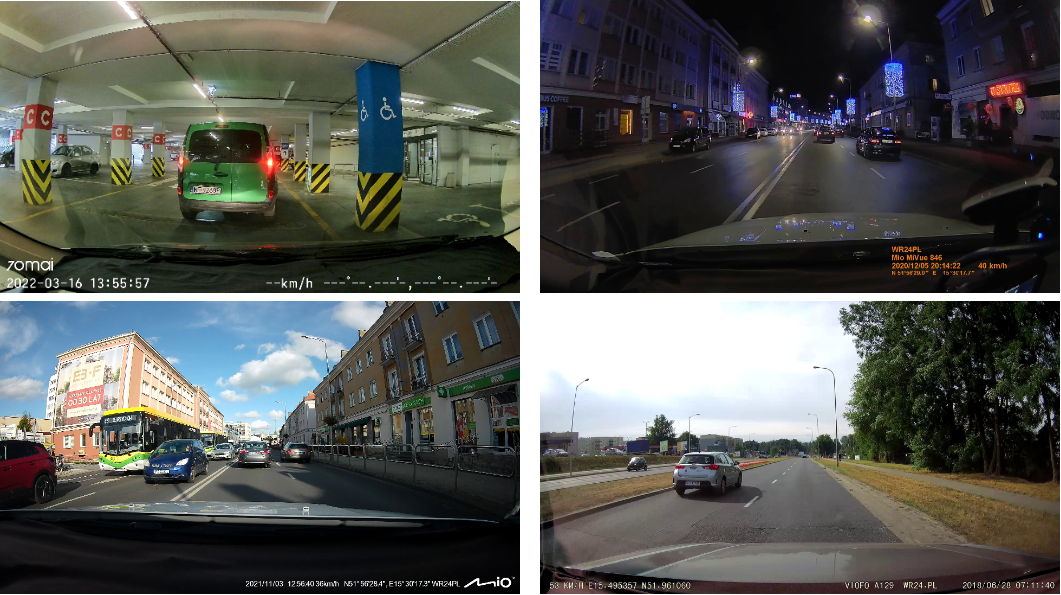
\includegraphics[scale=0.4]{Pictures/captured_frames}
    \caption{Pozyskane zdjęcia z wideorejestratora (źródło: opracowanie własne).}
    \label{fig:captured_frame}
\end{figure}
\FloatBarrier

Kolejnym krokiem niezbędnym przed rozpoczęciem procesu uczenia było nadanie etykiet obiektom na wyeksportowanych zdjęciach.
W tym celu opracowano skrypt służący do ręcznego oznaczania tablic rejestracyjnych.
Skrypt powstał na podstawie narzędzia~\cite{haar_object_marker}.
Jego fragment w postaci pseudokodu przedstawiono na poniższym schemacie.
\begin{algorithm}
    \caption{Procedura zapisująca współrzędne pozytywnych próbek.}
    \begin{algorithmic}[1]
        \label{create_positives}
        \Procedure{ObjectMarkerOnClick}{$(event, x, y)$}
            \If{$event == $ kliknięcie lewego przycisku myszy}
                \If {Liczba kliknięć jest nieparzysta}
                    \State Przypisz współrzędne $(x,y)$ kliknięcia jako początek obszaru próbki.
                \Else
                    \State Przypisz współrzędne $(x,y)$ kliknięcia jako koniec obszaru próbki.
                    \State Zwiększ liczbę obiektów w obrazie.
                    \State Przeskaluj współrzędne do stałej wartości.
                    \State Dodaj do listy pozytywów zaznaczony fragment.
                \EndIf
            \EndIf
        \EndProcedure
    \end{algorithmic}
\end{algorithm}
\FloatBarrier


%\begin{lstlisting}[language=Python, caption=Funkcja do oznaczania fragmentów obrazu zawierających poszukiwany obiekt., label=alg:positive_creator]
%import cv2
%
%def obj_marker(event, x, y):
%    global click_count
%    global debug
%    global obj_list
%    global obj_count
%    global frameName
%    global x1
%    global y1
%    global w
%    global h
%    global frame
%    global frameResized
%    if event == cv2.EVENT_LBUTTONDOWN:
%        click_count += 1
%        if click_count % 2 == 1:
%            x1 = x
%            y1 = y
%        else:
%            orgShape = frame.shape
%            ratioH = orgShape[0] / 1080
%            ratioW = orgShape[1] / 1920
%
%            w = abs(x1 - x)
%            h = abs(y1 - y)
%            obj_count += 1
%            if x1 > x:
%                x1 = x
%            if y1 > y:
%                y1 = y
%            obj_list.append('%d %d %d %d ' % (x1 * ratioW, y1 * ratioH, w * ratioW, h * ratioH))
%            cv2.rectangle(frameResized, (x1, y1), (x1 + w, y1 + h), (0, 255, 0), 1)
%            cv2.imshow(frameName, frameResized)
%\end{lstlisting}
Wszystkie zdjęcia wyświetlano po kolei na ekranie.
Zdarzenie kliknięcia myszką na obrazie przechwytywano w programie.
Pierwsze kliknięcie oznaczało współrzędne początku obszaru pozytywnej próbki.
Drugie kliknięcie oznaczało współrzędne końca rozpatrywanego obszaru.
Jak wspomniano wcześniej, obrazy posiadały różne rozdzielczości, często przewyższające rozdzielczość monitora.
Aby zdjęcia wyświetlały się poprawnie, skalowano je do rozdzielczości ekranu, na którym przeprowadzono operację nadawania etykiet.
Pozyskane koordynaty zapisywano do globalnej tablicy.
Na koniec procesu dane zapisano do pliku tekstowego, z którego odczytywano dane podczas etapu uczenia.
Dane w pliku zapisano w formacie \textit{ścieżka do pliku, liczba obiektów w pliku, kolejno współrzędne każdego z prostokątów}.
W Tabeli~\ref{tab:tab_data_set_characteristics} przedstawiono cechy charakterystyczne przygotowanego zbioru.
\begin{table}[h]
    \centering
    \caption{Parametry opracowanego zbioru.}
    \begin{tabular}{l l l}
        \toprule
        \textbf{Parametr}                      & \textbf{Wartość}                                     \\
        \midrule
        Liczba zdjęć                           & 10985                                                \\
        Format zdjęć                           & JPG                                                  \\
        Liczba zdjęć zawierających tablice     & 5248                                                 \\
        Ogółem liczba tablic                   & 10301                                                \\
        Zakres liczby tablic na jednym zdjęciu & 0--6                                                 \\
        Średnia wysokość próbki                & 38px                                                 \\
        Średnia szerokość próbki               & 91px                                                 \\
        Maksymalne rozmiary próbki             & 378$\times$136px                                     \\
        Minimalne rozmiary próbki              & 15$\times$11px                                       \\
        Rozdzielczości zdjęć                   & 1920$\times$1080, 2560$\times$1440, 3840$\times$2160 \\
        Liczba klatek na sekundę               & 30 kl/s, 60 kl/s                                     \\
        \bottomrule
    \end{tabular}
    \label{tab:tab_data_set_characteristics}
\end{table} % chapter2.tex zawiera treść rozdziału 2
    %----------------------------------------------------------------------------------------
%	CHAPTER 3
%----------------------------------------------------------------------------------------

\chapter{Opracowany algorytm}
\label{ch:opracowany-algorytm}
\chaptermark{Opracowany algorytm}
W przedstawionej pracy zrealizowano program rozpoznający tablice rejestracyjne na sekwencjach wideo pochodzących z kamery samochodowej.
Do detekcji użyto skanowania obrazu oknem przesuwnym i klasyfikowanie na podstawie cech Haara za pomocą algorytmu RealBoost.
Jako słaby klasyfikator wykorzystano algorytm koszykowania wartości funkcją logit.
Rozpoznane fragmenty obrazu zawierające tablice poddano operacjom morfologicznym.
Z przetworzonych obrazów segmentowano znaki tablicy rejestracyjnej.
Do rozpoznania znaków użyto biblioteki Tesseract opartej o rekurencyjne sieci neuronowe LSTM\@.


\section{Proces uczenia klasyfikatora}
\label{sec:proces-uczenia-klasyfikatora}
Proces uczenia klasyfikatora jest kluczowym etapem budowy modelu uczenia maszynowego.
Jeżeli na tym etapie dojdzie do błędu, będzie to rzutować na działanie całej aplikacji.
Częstym zjawiskiem w uczeniu maszynowym jest przeuczenie (ang. \textit{overfitting}).
Polega ono na wykrywaniu pozornych prawidłowości w dużej ilości danych, gdzie prawdziwe prawidłowości są prostsze lub słabsze, lub są maskowane przez błędy, lub są całkowicie nieistniejące~\cite{overfitting}.
Innym niepożądanym przypadkiem błędnego wyuczenia jest niedouczenie (ang. \textit{underfitting}).
Wynika ono najczęściej z zastosowania zbyt uproszczonego modelu lub niewystarczającej liczby próbek uczących~\cite{overfitting}.
Mając powyższe na uwadze, należy przyłożyć staranną uwagę do przygotowania odpowiedniego zbioru uczącego.
Nieprawidłowości na tym etapie będą bardzo trudno do wyeliminowania w późniejszych częściach systemu.

\subsection{Przygotowanie danych uczących}
\label{subsec:przygotowanie-danych-uczacych}
W rozdziale~\ref{ch:preparing_data_set} przedstawiono opracowany zbiór zdjęć z kamery samochodowej zawierający poruszające się pojazdy wraz z ich tablicami rejestracyjnymi.
Klasyfikatory działają jednak w inny sposób niż ludzki mózg i wymagają innych wartości, na których będą mogły podejmować decyzje.
W niniejszej pracy zdecydowano się wykorzystać cechy Haara jako cechy reprezentujące poszukiwane obiekty.
W celu wyuczenia klasyfikatora, należało opracowany wcześniej zbiór przetworzyć, aby każda negatywna i pozytywna próbka miała swoją reprezentację liczbową.
Na Rysunku~\ref{fig:haar_feats_dataset_prepare} przedstawiono schemat blokowy procesu przygotowania danych uczących dla klasyfikatora.
\begin{figure}[!ht]
    \centering
    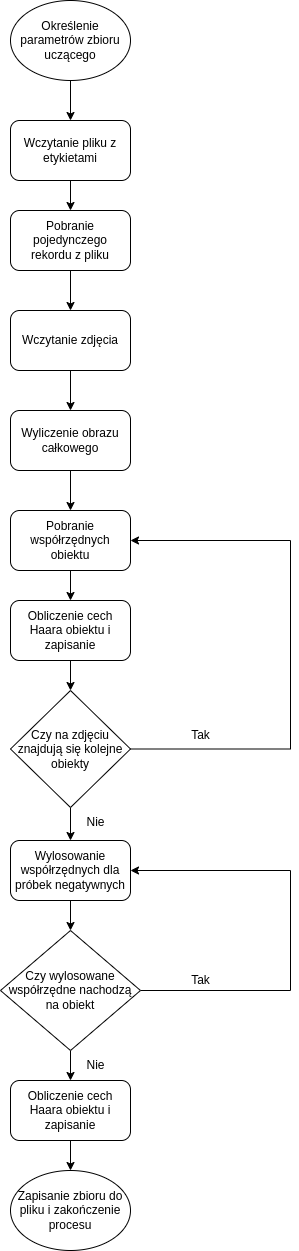
\includegraphics[scale=0.4]{Pictures/prepare_haar_dataset}
    \caption{Schemat blokowy przygotowania danych uczących dla klasyfikatora (źródło: opracowanie własne).}
    \label{fig:haar_feats_dataset_prepare}
\end{figure}
\FloatBarrier
Pierwszą czynnością jest określenie parametrów zbioru uczącego.
Przed rozpoczęciem uczenia należy określić ile cech ma być liczonych z jednej próbki.
Każdy szablon może być odpowiednią ilość razy skalowany wzdłuż każdego z kierunków.
Parametr ten oznacza się literą $s$.
Parametr $p$ oznacza rozmiary regularnej siatki ($(2p-1)\times (2p-1)$) punktów zaczepienia cech~\cite{szybka_detekcja_klesk}.
Na podstawie powyższych parametrów określa się liczbę cech niezbędnych do wyliczenia w trakcie przetwarzania jednego okna wg wzoru~\eqref{eq:features_count}
\begin{equation}
    \label{eq:features_count}
    n(s,p)=6s^2(2p-1)^2.
\end{equation}
Przykładowo, dla $s=3$ i $p=4$ liczba niezbędnych do wyliczenia cech jest równa 2205.
Dla $s=p=5$ liczba ta rośnie do 10125.
Im większa jest liczba cech tym dokładność detekcji powinna rosnąć.
Jednak wraz ze wzrostem liczby cech, rośnie również czas wykonania skryptu ze względu na większą liczbę niezbędnych do wykonania obliczeń.
Innym wejściowym parametrem jest ustalenie stosunku próbek pozytywnych do próbek negatywnych.

Po ustaleniu wejściowych parametrów, wczytywany jest plik tekstowy ze współrzędnymi tablic dla konkretnych plików.
Dla każdego rekordu w zbiorze, wczytywane jest odpowiednie zdjęcie.
Następnie algorytm iteruje po wszystkich pozytywnych próbkach znajdujących się w rozpatrywanym pliku.
Dla każdej próbki wyliczane są cechy Haara za pomocą wygenerowanych wcześniej szablonów.

W opisywanym programie użyto 5 szablonów cech Haara.
Szablony są skalowane odpowiednim skokiem zależnym od $s$.
Poniżej zamieszczono kod procedury generującej współrzędne szablonu dla każdej cechy~\ref{lst:haar_cords}.
\begin{lstlisting}[language=Python, caption=Procedura generujące szablony cech Haara dla konkretnych wpsółrzędnych., label={lst:haar_cords}]
def haar_coords(s, p, indexes):
    coords = []
    f_jump = (FEATURE_MAX - FEATURE_MIN) / (s - 1)
    for t, s_j, s_k, p_j, p_k in indexes:
        f_h = FEATURE_MIN + s_j * f_jump
        f_w = FEATURE_MIN + s_k * f_jump
        p_jump_h = (1.0 - f_h) / (2 * p - 2)
        p_jump_w = (1.0 - f_w) / (2 * p - 2)
        pos_j = 0.5 + p_j * p_jump_h - 0.5 * f_h
        pos_k = 0.5 + p_k * p_jump_w - 0.5 * f_w
        single_coords = [np.array([pos_j, pos_k, f_h, f_w])]  # whole rectangle for single feature
        for white in HAAR_TEMPLATES[t]:
            white_coords = np.array([pos_j, pos_k, 0.0, 0.0]) + white * np.array([f_h, f_w, f_h, f_w])
            single_coords.append(white_coords)
        coords.append(np.array(single_coords))
    return np.array(coords, dtype=object)
\end{lstlisting}
Na Rysunku~\ref{fig:haar_feats_examples} pokazano przykładowe szablony podczas procesu uczenia.
\begin{figure}[!ht]
    \centering
    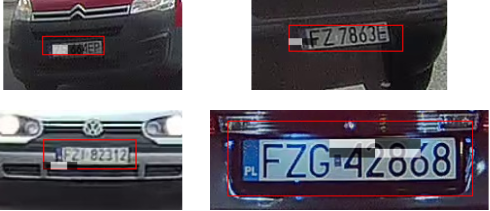
\includegraphics[scale=0.6]{Pictures/haar_tepmplates}
    \caption{Ekstrakcja cech za pomocą obrazów całkowych (źródło: opracowanie własne).}
    \label{fig:haar_feats_examples}
\end{figure}
\FloatBarrier

Po przeprocesowaniu wszystkich pozytywnych próbek, algorytm generuje negatywy.
Negatywne próbki są generowane losowo.
Losowana jest szerokość okna jako wartość w przedziale od 1 do 10 procent szerokości całego obrazu.
Wysokość okna jest zależna od szerokości.
Przyjęto, że wysokość okna powinna być równa $\dfrac{1}{3}, \dfrac{1}{4}$ lub $\dfrac{1}{5}$ szerokości.
Następnie dane są zapisywane do pliku.
W ten sposób przygotowane dane w następnym etapie posłużą do wyuczenia klasyfikatora.

\subsection{Uczenie klasyfikatora}
W niniejszej pracy zaimplementowano i wykorzystano algorytm wzmacniający RealBoost oparty o koszykowanie wartości funkcji logit.
Zasadę działania algorytmu RealBoost opisano szerzej w rozdziale~\ref{subsec:klasyfikatory}.
Na wejściu metody uczącej, funkcja przyjmuje cechy uczące oraz ich etykiety.
Dla każdej cechy obliczane są wartości maksymalne i minimalne.
Ustalane są one poprzez posortowanie wartości konkretnej cechy ze wszystkich próbek ze zbioru uczącego.
Algorytm dodaje odpowiedni margines, aby odrzucić skrajne wyniki.
Współczynnik ten ustalono na poziomie $0.05$.
Oznacza to, że dla zbioru o wielkości 100 próbek, odrzucone zostanie 5 pierwszych i 5 ostatnich wartości cech do wyznaczenia wartości brzegowych.
Następnie przypisywane są indeksy koszyków do poszczególnych cech.
Kolejnym krokiem jest przygotowanie indeksów, które przechowują informację o tym czy cecha dla konkretnego koszyka powiązana jest z próbką pozytywną czy negatywną.
Po przygotowaniu powyższych danych, algorytm przechodzi do wybrania najważniejszych cech z punktu widzenia klasyfikatora.
Obliczane jest to poprzez iterację po wszystkich cechach i określeniu cechy dla każdego klasyfikatora o najmniejszym błędzie.
Wyznaczane jest to za pomocą funkcji logit, która jest wyznaczana dla każdego z koszyków \\z osobna.
Na koniec dochodzi do reważenia wag.
Czynność jest powtarza dla każdego słabego klasyfikatora.
Algorytm~\ref{lst:fit_realboostbins} ukazuje fragment metody uczącej odpowiedzialny za wyliczenie odpowiedzi dla każdego ze słabych klasyfikatorów i wyznaczenie indeksów najlepszych cech.\\\\\\\\\\
\begin{lstlisting}[language=Python, caption=Procedura ucząca klasyfikator RealBoostBins., label={lst:fit_realboostbins}]
w = np.ones(m) / m
for t in range(self.T_):
    j_best = None
    logits_best = None
    err_exp_best = np.inf
    for j in range(n):
        logits = np.zeros(self.B_)
        for b in range(self.B_):
            W_positive = w[indexer_positive[j, b]].sum()
            W_negative = w[indexer_negative[j, b]].sum()
            logits[b] = self.logit(W_positive, W_negative)
        err_exp = np.sum(w * np.exp(-yy * logits[X_binned[:, j]]))
        if err_exp < err_exp_best:
            err_exp_best = err_exp
            logits_best = logits
            j_best = j
    self.feature_indexes_[t] = j_best
    self.logits_[t] = logits_best
    w = w * np.exp(-yy * logits_best[X_binned[:, j_best]])
    w /= err_exp_best

\end{lstlisting}
Na Rysunku~\ref{fig:fit_realboostbins} przedstawiono schemat blokowy uczenia klasyfikatora.
\begin{figure}[!ht]
    \centering
    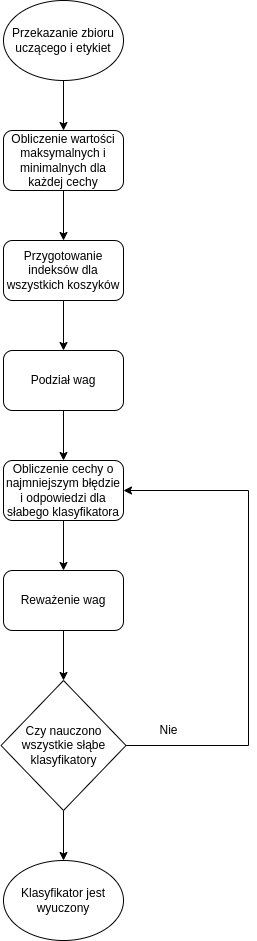
\includegraphics[scale=0.4]{Pictures/fit_realboostbins}
    \caption{Schemat blokowy funkcji uczącej klasyfikatora RealBoostBins (źródło: opracowanie własne).}
    \label{fig:fit_realboostbins}
\end{figure}
\FloatBarrier


\section{Schemat algorytmu}

Główną część programu można podzielić na dwa osobne moduły.
Pierwszy z nich odpowiedzialny jest za detekcję tablic na obrazie wejściowym.
Drugi moduł odpowiada za segmentację i rozpoznawanie znaków.
Przed rozpoczęciem detekcji, obraz jest skalowany.
W opracowanym algorytmie, ustalono wysokość na poziomie 480px.
Szerokość obrazu była proporcjonalnie skalowana.
Następnie obraz konwertowano do skali szarości.
Przed rozpoczęciem detekcji oknem przesuwnym, obliczano obraz całkowy.
Szablony cech Haara ograniczono tylko do tych odpowiadających cechom wybranym przez słabe klasyfikatory na etapie uczenia klasyfikatora.
Na Rysunku~\ref{fig:main_alg} przedstawiono schemat blokowy algorytmu rozpoznawania tablic rejestracyjnych.
\begin{figure}[!ht]
    \centering
    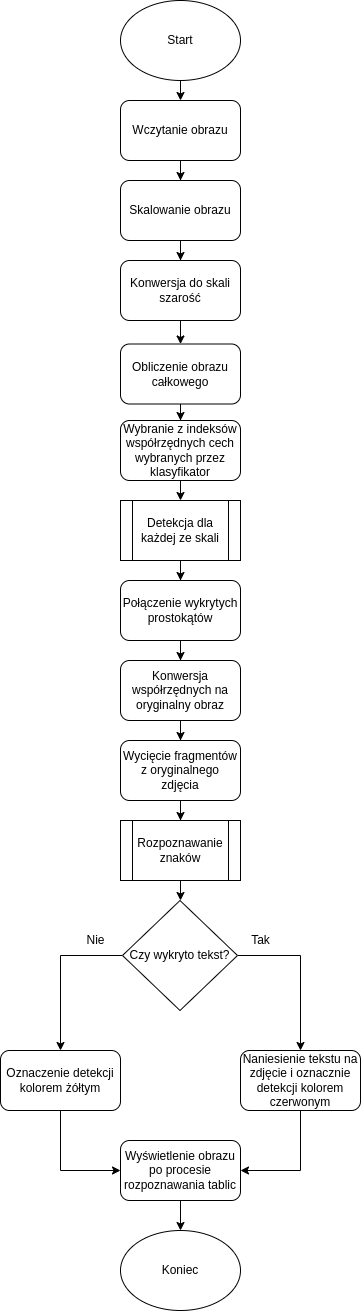
\includegraphics[scale=0.4]{Pictures/main_alg}
    \caption{Schemat blokowy algorytmu rozpoznawania tablic rejestracyjnych (źródło: opracowanie własne).}
    \label{fig:main_alg}
\end{figure}
\FloatBarrier

\subsection{Algorytm detekcji}
Algorytm detekcji odpowiada za zlokalizowanie obszarów potencjalnie zawierających tablice rejestracyjne.
Mając na uwadze fakt, że tablice mogą mieć różne rozmiary na zdjęciu, dla procedury skanującej oknem przesuwnym należało zastosować kilka skal okna.
Okno przesuwano w obrazie odpowiednim skokiem w poziomie oraz w pionie.
Poziomy skok $d_w$ obliczano na podstawie wzoru~\eqref{eq:jump_detect_window}
\begin{equation}
    \label{eq:jump_detect_window}
    d_w = \round(w * \lambda),
\end{equation}
gdzie $w$ jest szerokością okna, a $\lambda$ oznacza współczynnik przemieszczania okna.
Skok pionowy wyznaczano w analogiczny sposób.
Dla każdego okna obliczano cechy Haara dla indeksów wyznaczonych podczas procesu uczenia klasyfikatora.
Następnie obliczano odpowiedź klasyfikatora.
Jeśli była ona większa od podanego progu, okno oznaczano jako pozytywne.
Na Rysunku~\ref{fig:detection_alg} przedstawiono schemat blokowy algorytmu detekcji tablic rejestracyjnych.
\begin{figure}[!ht]
    \centering
    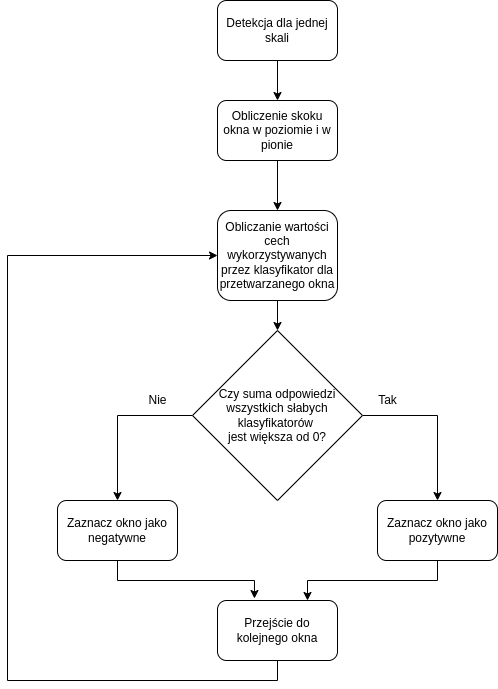
\includegraphics[scale=0.35]{Pictures/detection_alg}
    \caption{Schemat blokowy algorytmu detekcji tablic rejestracyjnych (źródło: opracowanie własne).}
    \label{fig:detection_alg}
\end{figure}
\FloatBarrier
Po wykonaniu procedury skanowania oknem przesuwnym, rozpoczęto przetwarzanie okien oznaczonych jako pozytywne.
Z uwagi na fakt, że w otoczeniu tablicy rejestracyjnej wiele okien mogło zostać oznaczonych jako pozytywne, należało te okna połączyć.
Dzięki temu moduł rozpoznawania znaków otrzyma znacznie mniejszą ilość okien.
W kolejnym kroku współrzędne połączonych okien konwertowano do współrzędnych w oryginalnym obrazie.
Taka operacja ma na celu przekazanie do modułu OCR fragmentu obrazu w jakości równej obrazowi sprzed procedury skalowania.
Rysunek~\ref{fig:non_max_supression} przedstawia porównanie procedury detekcji bez oraz z zastosowaniem techniką łączenia okien.
Do połączenia okien zastosowano algorytm usuwania niemaksymalnych pikseli (ang. \textit{non-maximum suppression}).
\begin{figure}[!ht]
    \centering
    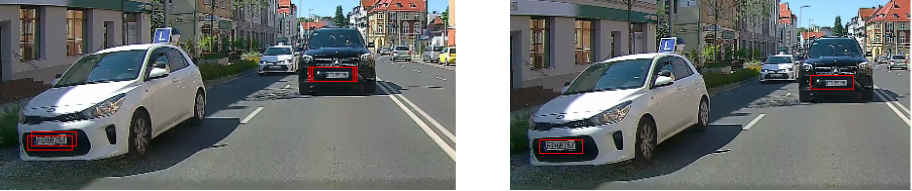
\includegraphics[scale=0.4]{Pictures/non_max_supression}
    \caption{Porównanie detekcji tablicy rejestracyjnej bez i z zastosowaniem algorytmu łączenia okien (źródło: opracowanie własne).}
    \label{fig:non_max_supression}
\end{figure}
\FloatBarrier

\subsection{Algorytm segmentacji i rozpoznawania znaków}
Moduł odpowiedzialny za rozpoznawanie znaków otrzymuje na wejściu wycięty fragment obrazu w oryginalnej jakości.
Następnie przed rozpoczęciem segmentacji znaków, obraz jest skalowany do wysokości 300px.
W kolejnym kroku, obraz jest konwertowany do modelu barw w skali szarości.
W celu segmentacji znaków, zaproponowano podejście łączące dwie techniki.
Zdecydowano się na takie rozwiązanie, ponieważ zauważono, że wzajemnie się one uzupełniają i ich połączenie daje lepsze wyniki.
Pierwsza z technik polegała na binaryzacji obrazu z wykorzystaniem metody Otsu.
Na tak przygotowanym obrazie wykryto kontury korzystając z metody z biblioteki OpenCV \textit{findContours}.
Druga technika wykorzystywała maskę binarną w przestrzeni barw HSV\@.
Następnie przetworzony obraz poddawano operacjom morfologicznym.
Wynikowy obraz przekazano do metody wykrywającej kontury.

Metoda \textit{findContours} przyjmuje parametr $mode$, który odpowiada za sposób selekcji konturów.
Procedura może zwracać np.\ tylko kontury zewnętrzne lub wewnętrzne lub zwracać strukturę hierarchiczną~\cite{open_cv_contours_mode}.
W opisywanym rozwiązaniu wybrano opcje \textit{RETR\_TREE}, która pobiera wszystkie kontury i rekonstruuje pełną hierarchię zagnieżdżonych konturów.
W \textit{findContours} możliwa jest również do wybrania metoda aproksymacji konturów.
Dla wartości \textit{CHAIN\_APPROX\_NONE} zbierane są wszystkie wartości konturów.
Dla wartości \textit{CHAIN\_APPROX\_SIMPLE} algorytm kompresuje poziomie, pionowe oraz diagonalne segmenty i pozostawia tylko punkty końcowe.
Zdecydowano się na drugą metodę aproksymacji.

Dla obu podejść zbiory wykrytych konturów połączono w całość.
Wykryte kontury należało przefiltrować, w celu wybrania tylko tych odpowiadającym znakom na tablicy rejestracyjnej.
Opracowano procedurą z następującymi krokami:
\begin{enumerate}
    \item pobranie prostokąta otaczającego dany kontur,
    \item odrzucenie konturu, jeśli wysokość prostokąta jest większa od wysokości obrazu pomniejszonej o stałą wartość
    \item obliczenie powierzchni prostokąta,
    \item odrzucenie konturu, jeśli powierzchnia jest mniejsza od stałej wartości,
    \item odrzucenie konturu, jeśli stosunek boków prostokąta jest spoza przyjętego zakresu.
\end{enumerate}
Na podstawie powyższej procedury odrzucono część wykrytych wcześniej konturów.
Korzystając z założenia, że wszystkie znaki na tablicy rejestracyjnej są takiej samej wysokości, odrzucono z powstałego zbioru kontury, których wysokość najbardziej odbiegała od średniej wysokości całego zbioru.
Ostateczny zbiór konturów posłużył do wycięcia znaków ze zbinaryzowanego obrazu.
W ten sposób przeprowadzono segmentację znaków.
Nowy obraz, z oddzielonymi znakami od tła, przekazano do biblioteki Tesseract.
Skorzystano z metody \textit{image\_to\_string}, która zwraca tekst na podstawie obrazu wejściowego.
Na Rysunku~\ref{fig:characters_alg} przedstawiono schemat blokowy algorytmu rozpoznawania znaków.
\begin{figure}[!ht]
    \centering
    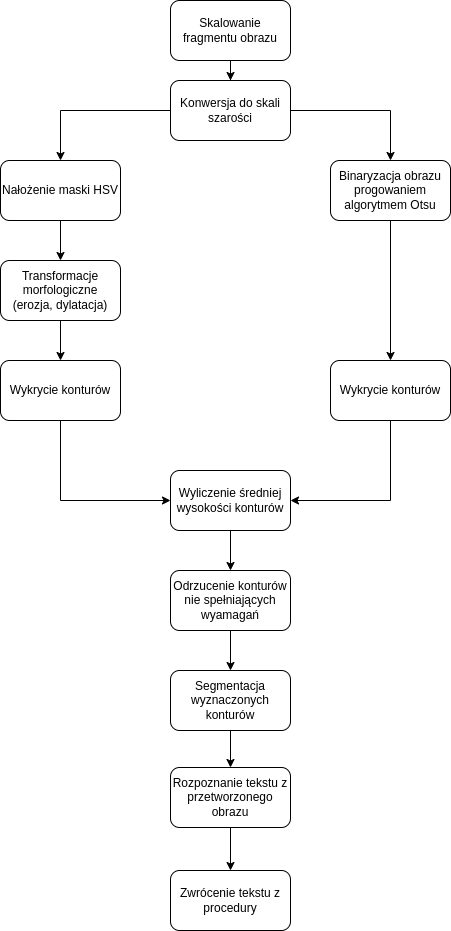
\includegraphics[scale=0.4]{Pictures/characters_alg}
    \caption{Schemat blokowy algorytmu rozpoznawania tablic (źródło: opracowanie własne).}
    \label{fig:characters_alg}
\end{figure}
\FloatBarrier
Na Rysunku~\ref{fig:segmentation} przedstawiono przykładowy proces segmentacji znaków.
Pierwszy obraz jest obrazem wejściowym, który trafił do algorytmu z detektora tablic rejestracyjnych.
Ostatni obraz jest wynikiem segmentacji.
Obraz środkowy jest obrazem wejściowym, na który nałożono wykryte pozycje znaków (kolor niebieski).
Kolorem różowym oznaczono kontury, które zostały wykryte, ale zostały odrzucone z powodu braku spełnienia kryteriów geometrycznych.
Założono, że kontur musi być prostokątem o dłuższych bokach zorientowanych w pionie.
Kolorem żółtym oznaczono kontury, które zostały odrzucone, z powodu ich zbyt dużego odchylenia od średniej wysokości konturów.
\begin{figure}[!ht]
    \centering
    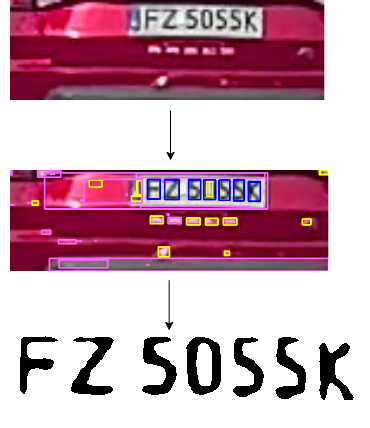
\includegraphics[scale=0.4]{Pictures/segmentation}
    \caption{Proces segmentacji znaków (źródło: opracowanie własne).}
    \label{fig:segmentation}
\end{figure}
\FloatBarrier


\section{Biblioteki użyte w programie}
Środowisko Python jest niezwykle popularne m.in. ze względu na mnogość dostępnych gotowych bilbiotek.
Jednym z celów pracy było zaimplementowanie algorytmu uczącego i klasyfikującego.
Cel ten udało się zrealizować, natomiast nie byłoby to możliwe bez użycia gotowych rozwiązań do elementarnych operacji t.j. listowanie plików w katalogach, odczyt i zapis zdjęć, pobieranie pojedynczych klatek z filmu wideo czy operacje na tablicach.
Poniżej wymieniono i opisano najważniejsze oraz najczęściej używane biblioteki w opisywanej pracy.

\subsection{OpenCV}
OpenCV jest biblioteką o otwartym źródle (ang. \textit{open source}) \cite{open_cv,open_cv_docs} .
Do jej głównych zastosowań należą przetwarzanie obrazów oraz uczenie maszynowe.
W przedstawionym programie wykorzystano najnowszą dostępną wersję na moment pisania pracy $4.6.0$.
Została zaprojektowana, aby zapewnić ustandaryzowaną infrastrukturę dla aplikacji widzenia komputerowego.
Oprogramowanie dystrybuowane jest na licencji BSD.
Pierwsza wersja została opracowana w roku 1999.
Oryginalnie powstała w języku C++, natomiast istnieją biblioteki pozwalające używać jej w innych językach programowania.
Bibliotekę można podzielić na kilka głównych modułów:
\begin{itemize}
    \item przetwarzanie obrazów - moduł zawiera zestaw metod do przeprowadzania takich operacji jak filtrowanie, przekształcenia geometryczne, zmiana przestrzeni kolorów, histogramy,
    \item przetwarzanie wideo - zestaw metod, które pozwalają na m. in. usuwanie tła, śledzenie obiektów, wykrywanie ruchu,
    \item operacje wejścia/wyjścia na wideo - wyciąganie poszczególnych klatek z wideo, kodowanie, zapis i odczyt wideo,
    \item HighGUI - moduł służący do wizualizacji wyników, wyświetlania okien, zaznaczania ROI (ang. \textit{Region of interest}).
\end{itemize}

Poniżej wymieniono użyte w stworzonym programie funkcje wraz z krótkim opisem ich zastosowania:
\begin{itemize}
    \item \textit{videoCapture} - przechwytywanie obrazów z pliku wideo,
    \item \textit{cvtColor} - zmiana przestrzeni barw w obrazie,
    \item \textit{imread} - wczytanie obrazu z pliku,
    \item \textit{imshow} - wyświetlenie obrazu,
    \item \textit{imwrite} - zapis obrazu do pliku,
    \item \textit{rectangle} - rysowanie prostokąta na obrazie,
    \item \textit{putText} - umiejscowienie tekstu na obrazie,
    \item \textit{addWeighted} - połączenie dwóch obrazów poprzez nałożenie ich na siebie,
    \item \textit{thresholding} - binaryzacja obrazu,
    \item \textit{GaussianBlur} - wygładzanie obrazu za pomocą funkcji Gaussa,
    \item \textit{Canny} - wykrywanie krawędzi za pomocą algorytmu Johna F. Canny'ego \cite{4767851},
    \item \textit{findContours} - wykrywanie konturów obiektów (punktów o tym samym kolorze lub intensywności łączących się w krzywe),
    \item \textit{resize} - zmiana wielkości obrazu,
    \item \textit{imdecode} - odczytywanie zdjęcia z bufora.
\end{itemize}

\subsection{Tesseract OCR}
Biblioteka Tesseract jest pakietem składającym się z programu lini poleceń \textit{tesseract} oraz silnika OCR \textit{libtesseract}~\cite{tesseract}.
Tesseract powstał między rokiem 1985, a 1994 na potrzeby firmy Hewlett-Packard.
W roku 2005 firma upubliczniła bibliotekę jako rozwiązanie \textit{open-source}.
Od początku 2006 do listopada 2018 za rozwój Tesseract odpowiedzialna była firma Google.
Obecnie głównym programistą projektu jest Ray Smith.
Silnik programu oparty jest o język programowania C++.
W celu wykorzystania jej w opisywanym programie, użyto nakładki \textit{pytesseract}~\cite{pytesseract}.
Autorzy deklarują, że najnowsza wersja 5, wydana w listopadzie 2021, wspiera ponad 100 języków.
Biblioteka wykorzystuje rekurencyjne sieci neuronowe LSTM (ang. \textit{Long Short-Temp Memory})~\cite{lstm}.

\subsection{NumPy}
Biblioteka NumPy jest jednym z fundamentalnych pakietów dla obliczeń naukowych \\w środowisku Python~\cite{numpy}.
Głównym elementem biblioteki jest obiekt \textit{ndarray}.
Obiekt ten pozwala na tworzenie wielowymiarowych tablic o ściśle określonym typie danych.
Oprócz tego, biblioteka zapewnia wiele operacji matematycznych do wykonania na tablicach.
Operacje wykonywane za pomocą biblioteki NumPy są znacznie bardziej wydajne od standardowych metod języka Python.
Dzieję się tak, ponieważ biblioteka posiada zaimplementowane metody w języku C\@.
W opisywanym programie, dzięki zastosowaniu NumPy m.in.\ do obliczenia obrazu całkowego za pomocą metody \textit{cumsum}, osiągnięto znacznie większą wydajność w tym zakresie.

\subsection{Pickle}
Moduł Pickle wchodzi w skład podstawowego pakietu Python.
Jego zastosowaniem jest serializacja danych.
Dzięki temu, możliwe jest zapisanie dowolnego obiektu i jego późniejsze odczytanie.
W trakcie opracowywania niniejszego oprogramowania, operacja ta była niezwykle przydatna.
Dzięki temu rozwiązaniu, możliwe było np.\ wczytanie \\z pliku nauczonego klasyfikatora.
Biblioteka jest niezwykle prosta w użyciu.
Korzystając z bibliotek do serializacji, należy mieć na uwadze fakt, że wczytywanie zserializowanych obiektów może prowadzić do naruszenia zasad bezpieczeństwa programu.
Z tego powodu, należy wczytywać tylko takie obiekty, których pochodzenia użytkownik jest pewien.

\subsection{Numba}
Numba jest biblioteką służącą do poprawiania wydajności programów napisanych w języku Python.
Pakiet kompiluje kod w trakcie trwania programu (ang. \textit{just in time} --- JIT), w celu zwiększenia jego wydajności.
Operacja ta jest działa najlepiej dla kodu opartego o tablice NumPy, pętle i funkcje.
W celu kompilacji, fragmenty kodu oznacza się specjalnymi adnotacjami.
Po natrafieniu na odpowiednią komendę, biblioteka kompiluje \\w trakcie trwania programu kod do postaci kodu maszynowego, dzięki czemu wydajność skompilowanego fragmentu jest porównywalna do wykonywania kodu maszynowego~\cite{numba}.

\subsection{Joblib}
Biblioteka Joblib zapewnia zestaw narzędzi do zarządzaniem przepływem (ang. \textit{flow}) kodu w programach napisanych w języku w Python.
W opisywanym rozwiązaniu wykorzystano moduł Parallel do równoległego wykonywania kodu.
Poza tym, Joblib oferuje cache'owanie danych oraz ich leniwe ładowanie (ang. \textit{lazy loading}).
Jednymi z istotnych zalet jest brak zależności do innych niestandardowych pakietów oraz wysoka wydajność na dużych zbiorach danych. % chapter2.tex zawiera treść rozdziału 2
    %----------------------------------------------------------------------------------------
%	CHAPTER 4
%----------------------------------------------------------------------------------------

\chapter{Wyniki badań}
\chaptermark{Wyniki badań} % Tekst, który wyświetli się w nagłówku strony,  jeżeli jest za długi tytuł rozdziałuchapter2.te
Do przeprowadzenia testów aplikacji wykorzystano komputer przenośny Dell Vostro 5515.
Komputer wyposażony został w 32GB pamięci RAM oraz procesor AMD Ryzen 5700u.
Bazowe taktowanie procesora było równe 1.8GHz, natomiast w trybie boost taktowanie rosło do 4.3GHz.
Procesor wyposażono w 8 rdzeni i 16 wątków.
Program testowano na systemie operacyjnym Ubuntu 20.04.5 LTS\@.


\section{Wyniki detekcji tablic rejestracyjnych}
W celu oceny dokładności klasyfikatora służącego do detekcji tablic rejestracyjnych, przygotowano zbiór testowy.
W zbiorze testowym znajdowało się 100 próbek pozytywnych oraz 10000 próbek negatywnych.
Wyniki dla poszczególnych klasyfikatorów przedstawia Tabela~\ref{tab:accuracy_clf}.

%\\opis przeprowadzony testów
%\\zrzuty z nagrań
%\\czasy
%\\wyraportowanie błędów
\begin{table}[h]
    \centering
    \caption{Dokładność klasyfikatorów w zadaniu klasyfikacji obrazów z tablicami rejestracyjnymi.}
    \label{tab:accuracy_clf}
    \begin{tabular}{c c c c c c}
        \toprule
        \textbf{\thead{Liczba \\cech}} & \textbf{\thead{Liczba  \\słabych \\klasyfikatorów}} & \textbf{\thead{Liczba \\koszyków}} & \textbf{\thead{Dokładność \\klasyfikatora}} & \textbf{\thead{Dokładność \\klasyfikatora dla \\próbek pozytywnych}} & \textbf{\thead{Dokładność \\klasyfikatora dla \\próbek negatywnych}} \\
        \midrule
        2205 & 32 & 8 & 99.70\% & 75.15\% & 99.94\% \\
        2205 & 64 & 8 & 99.77\% & 82.24\% & 99.94\% \\
        2205 & 256 & 8 & 99.87\% & 91.12\% & 99.96\% \\
        \bottomrule
    \end{tabular}
\end{table}
%\\można pokazać zdjęcia nocne
%\\duże tablice, małe tablice
%\\różny threshold, różne wyniki
%\\jako pozytywy wykrywane sa oznaczenia samochodów (modelu)
%\\reklamy i banery
%\\czas wykonywania
%\\krzywe roc
Z racji ograniczeń sprzętowych, nie udało się nauczyć klasyfikatorów dla okien \linebreak z większą ilością cech.

Poza zbiorem testowym, algorytm testowano na rzeczywistym nagraniu wideo pochodzącym z kamery samochodowej.
Poniżej przedstawiono wyniki dla tego rodzaju obrazów wejściowych.
Na wynikowych obrazach kolorem żółtym oznaczano okna, które klasyfikator oznaczył jako pozytywne dla progu $t$.
Kolorem czerwonym oznaczono okna, które zostały oznaczone jako pozytywne oraz udało się odczytać z nich tekst.

Na Rysunku~\ref{fig:tablica_rozpoznana} przedstawiono wyniki detekcji dla progu $t=1.5$.
Dla takiego obrazu, wykryto dwie tablice, z czego jedna została rozpoznana.
Po lewej stronie obrazu znajdują się jeszcze dwie kolejne tablice, jednak ich rozmiar jest znacznie mniejszy od wielkości okna przesuwnego.
Na obrazie można zauważyć wiele fałszywych pozytywów.
Biorąc pod uwagę cechy, którymi kieruje się klasyfikator, takie zaznaczenie nie jest bezpodstawne.
Przykładowo, zaznaczony został podpis pod znakiem zakazu wjazdu dla ciężarówek.
Tablica ta ma podobny kształt do tablicy rejestracyjnej oraz zawiera czarny tekst na białym tle.
Oprócz tego, po lewej stronie obrazu znajduje się duży szyld reklamowy zawieszony na ścianie budynku.
Zawiera on biały prostokąt z tekstem, co również jest problematyczne dla klasyfikatora.
\begin{figure}[!ht]
    \centering
    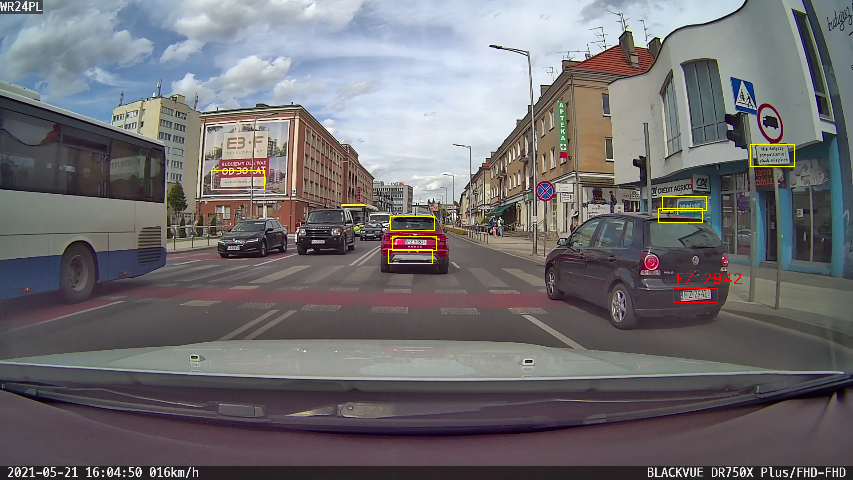
\includegraphics[scale=0.4]{Pictures/tablica_rozpoznana}
    \caption{Wyniki detekcji tablic rejestracyjnych dla progu $t=1.5$. Liczba cech $T=64$ (źródło: opracowanie własne).}
    \label{fig:tablica_rozpoznana}
\end{figure}
\FloatBarrier
Innym przykładem błędnej detekcji jest Rysunek~\ref{fig:autobus}.
Jako pozytyw oznaczono wyświetlacz autobusu, zawierający informację o numerze linii autobusowej.
\begin{figure}[!ht]
    \centering
    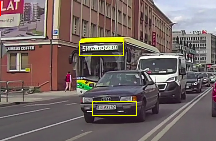
\includegraphics[scale=1]{Pictures/autobus}
    \caption{Wyświetlacz na autobusie wykryty jako tablica rejestracyjna dla progu $t=1.5$. Liczba cech $T=64$ (źródło: opracowanie własne).}
    \label{fig:autobus}
\end{figure}
\FloatBarrier
Kolejnym przykładem błędnej detekcji jest Rysunek~\ref{fig:bank}.
Jako pozytyw wykryto szyld banku.
Podobnie jak w przypadku wyświetlacza na autobusie, okno zawiera kontrastowy tekst.
\begin{figure}[!ht]
    \centering
    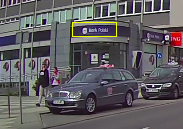
\includegraphics[scale=1]{Pictures/bank}
    \caption{Szyld reklamowy wykryty jako tablica rejestracyjna dla progu $t=1.5$. Liczba cech $T=64$ (źródło: opracowanie własne).}
    \label{fig:bank}
\end{figure}
\FloatBarrier
Z przedstawionymi błędami można walczyć za pomocą umiejętnego dobierania progu decyzyjnego $t$.
Dla progu $t=2.5$ powyższe okna nie zostają uznane za pozytywne.
Zwiększanie progu jednak objawia się również brakiem detekcji dla niektórych próbek prawdziwie pozytywnych.
Rysunek~\ref{fig:same_car} przedstawia problem braku detekcji tego samego samochodu pomiędzy klatkami.
Takie zachowanie wynika z nieprzekroczenia progu dla środkowego zdjęcia.
\begin{figure}[!ht]
    \centering
    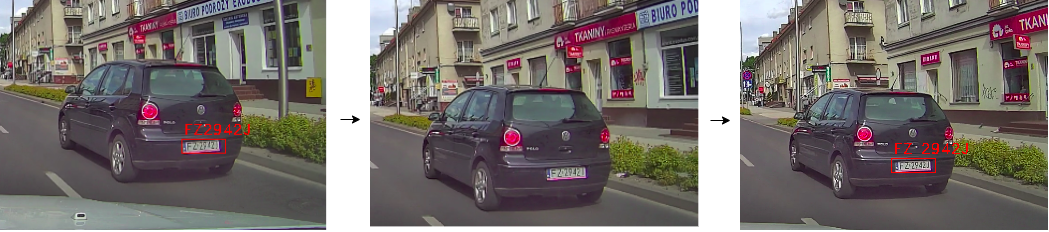
\includegraphics[scale=0.4]{Pictures/same_car}
    \caption{Brak detekcji tego samochodu pomiędzy klatkami dla progu $t=2.5$. Liczba cech $T=64$ (źródło: opracowanie własne).}
    \label{fig:same_car}
\end{figure}
\FloatBarrier
Warto również zaznaczyć fakt, że niektóre tablice są nieczytelne nawet dla ludzkiego oka.
Ludzki umysł niejako się domyśla, że z przodu lub z tyłu samochodu znajduje się tablica rejestracyjna, nawet jeżeli na zdjęciu bardziej przypomina biały prostokąt.
Opracowany klasyfikator nie ma takiej wiedzy.
Z tego powodu, określenie granicy, dla której próbki powinny być klasyfikowane jako pozytywne, nie jest trywialnym zadaniem.

Należy podkreślić, że procent poprawnie sklasyfikowanych próbek przez klasyfikator nie zawsze powinien być jedyną miarą jakości systemu.
Przykładowo, dla obrazu przedstawionego na Rysunku~\ref{fig:tablica_rozpoznana} procedura skanowania oknem przesuwnym, dla rozmiaru okna
45$\times$15px, generuje 39188 okien.
Jeżeli uznamy, że 20 okien zostało źle sklasyfikowanych, to poprawność klasyfikacji dalej jest bardzo wysoka i wynosi w tym przypadku $99.95\%$.


\section{Wyniki rozpoznawaniu znaków}
Jak wspomniano w poprzednim rozdziale, do rozpoznawania tekstu wykorzystano bibliotekę Tesseract.
Zgodnie z~\cite{sym12050715}, dokładność klasyfikacji biblioteki wynosi $70.2\%$.
\linebreak W rzeczywistości, jakość działania systemu w głównej mierze zależy od metod segmentacji znaków.
Na Rysunku~\ref{fig:plates} zaprezentowano przykładowe wyniki segmentacji znaków z tablic rejestracyjnych.
\begin{figure}[!ht]
    \centering
    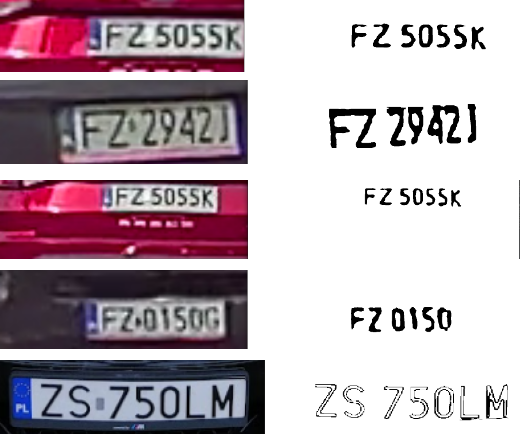
\includegraphics[scale=0.4]{Pictures/plates}
    \caption{Przykładowe wyniki segmentacji znaków z tablic rejestracyjnych (źródło: opracowanie własne).}
    \label{fig:plates}
\end{figure}
\FloatBarrier
Można przyjąć założenie, że im tablica jest większa, tym algorytm uzyskuje lepsze wyniki.
Wynika to przede wszystkim z mniejszych zakłóceń w obrazie i lepiej widocznych przerwach pomiędzy znakami.

Na jakość segmentacji i następnie odczytu znaków wpływ ma również rotacja tablicy rejestracyjnej.
Dodatkowo, w zależności od kąta, pod którym zrobiono zdjęcie, kontury znaków potrafią się łączyć ze sobą lub z ramką tablicy.
Ten fakt zdecydowanie nie ułatwia późniejszej segmentacji.
Śruby, które często stosowane są w celu zamocowania tablicy również negatywnie wpływają na segmentację znaków.
Mogą one powodować łączenie znaków i w konsekwencji zmianę ich konturów.

Zauważono, że jednym z problematycznych dla biblioteki znaków jest litera ,,J'', która często mylona była ze znakiem ,,)''.
Wykorzystując fakt, że tablice zawierają tylko znaki alfanumeryczne, można poprawić to programowo, poprzez zamianę tego znaku w rezultacie.
Trudniejszym do rozwiązania problemem jest wzajemne mylenie litery ,,S'' \linebreak z cyfrą 5.
Oba znaki mogą występować na tablicach rejestracyjnych.
Patrząc na przykładowe zdjęcia z Rysunku~\ref{fig:plates}, wyniki nie zawsze są oczywiste, nawet dla człowieka.

%\\przykłady:
%\\mylony znak ``('' z ``J''
%\\mylone S z 5


\section{Porównanie wydajności czasowej}
Dla systemów automatycznego rozpoznawania tablic rejestracyjnych wydajność jest jedną z kluczowych kwestii.
Aby dane mogły być odpowiednio przetwarzane, system powinien na bieżąco procesować zdjęcia.
Wydajność jest uzależniona od poniższych czynników:
\begin{itemize}
    \item rozmiar okna przesuwnego,
    \item liczba skal dla okna przesuwnego,
    \item liczba pozytywnych okien wysłanych do modułu rozpoznawania znaków,
    \item liczba cech klasyfikatora.
\end{itemize}
W Tabeli~\ref{tab:performance} przedstawiono wyniki uzyskanych czasów dla opracowanego programu.
W celu przyspieszenia obliczeń, zrównoleglono obliczenia cech dla procedury skanowania oknem przesuwnym.
Poniższe dane uwzględniają zrównloleglenie, stąd czas detekcji nie jest równy iloczynowi liczby okien i czasu klasyfikacji jednego okna.
Wszystkie obrazy były skalowane na wejściu do rozmiaru 640$\times$480px.
\begin{table}[h]
    \centering
    \caption{Wydajność czasowa systemu.}
    \label{tab:performance}
    \begin{tabular}{c c c c c c}
        \toprule
        \textbf{\thead{Liczba \\cech}} & \textbf{\thead{Liczba  \\unikalnych cech \\użytych przez \\ klasyfikator}} & \textbf{\thead{Liczba \\okien}} & \textbf{\thead{Czas \\detekcji}} & \textbf{\thead{Czas \\rozpoznawania \\jednej tablicy}} & \textbf{\thead{Czas przetwarzania \\jednego okna}} \\
        \midrule
        2205 & 32 & 39188 & 0.68s & 0.11s & 0.4ms \\
        2205 & 64 & 39188 & 0.91s & 0.12s & 0.9ms \\
        2205 & 256 & 39188 & 2.24s & 0.11s & 1.1ms \\
        \bottomrule
    \end{tabular}
\end{table}
Na podstawie zebranych danych, można zauważyć, że czas detekcji rośnie wraz ze wzrostem liczby używanych cech.
Czas rozpoznawania dla jednej tablicy jest stały (w granicach błędu pomiarowego).
Natomiast dla klasyfikatorów z większą liczbą cech, do modułu rozpoznawania znaków trafia mniej okien (z racji mniejszej ilości fałszywych pozytywów).
Z racji jednak większej ilości czasu poświęcanej podczas detekcji, zysk ten jest pomijalny.


\section{Propozycje udoskonalenia algorytmu}
Praca ma charakter eksperymentalny.
Opracowany program spełnia założenia detekcji tablic i rozpoznawania znaków na nich się znajdujących.
Z racji ograniczonego czasu oraz jednoosobowego zespołu, istnieją pola do ulepszeń w opracowanym systemie.

Jednym z pomysłów na udoskonalenie modułu detekcji jest dołożenie do zbioru uczącego negatywnych okien, które obecnie klasyfikator wykrywa błędnie, jako pozytywne.
Jest prawdopodobnym, że ponownie nauczony klasyfikator charakteryzowałby się wyższą dokładnością detekcji.
Innym pomysłem, który mógłby poprawić wydajność oraz jakość detekcji jest użycie więcej niż jednego klasyfikatora do detekcji obiektów.
W pierwszej kolejności jeden klasyfikator klasyfikowałby okna zawierający samochody.
Tak działający klasyfikator działby szybciej, ponieważ rozmiar okna w procedurze skanującej byłby większy.
Wynika to z faktu, że samochód zajmuje większy obraz na zdjęciu niż jego tablica rejestracyjna.
Następnie na wykrytych fragmentach należałoby wykryć tablice rejestracyjne.
W rezultacie liczba okien poddawanych procedurze predykcji mogłaby być mniejsza niż w oryginalnym rozwiązaniu.
Aby zwiększyć wydajność rozwiązania, możliwe jest również zaimplementowanie programu w silnie typowanym, kompilowanym języku, np.\ C++.

W celu poprawienia jakości rozpoznawania znaków, możliwe jest nauczenie sieci neuronowej biblioteki Tesseract zbiorem znaków z tablic rejestracyjnych.
Biblioteka domyślnie wyuczona jest na zbiorach znaków pochodzących z różnego rodzaju tekstów drukowanych, tj.\ książki lub dokumenty.
Podczas przygotowywania zbioru uczącego, szczególną uwagę należałoby przykuć do przygotowania znaków, które nie mają idealnych konturów.
Ma to na celu zapewnienie przykładów uczących maksymalnie zbliżonych do próbek w realnym środowisku pracy. % chapter2.tex zawiera treść rozdziału 2
%%%%%%%%%%%%%%%%%%%%%%%%%%%%%%%%%%%%%%%%%%
% Szablon pracy dyplomowej
% Wydział Informatyki 
% Zachodniopomorski Uniwersytet Technologiczny w Szczecinie
% autor Joanna Kołodziejczyk (jkolodziejczyk@zut.edu.pl)
% Bardzo wczesnym pierwowzorem szablonu był
% The Legrand Orange Book
% Version 2.1 (26/09/2018)
%
% Modifications to LOB assigned by %JK
%%%%%%%%%%%%%%%%%%%%%%%%%%%%%%%%%%%%%%%%%


%----------------------------------------------------------------------------------------
%	CHAPTER 2
%----------------------------------------------------------------------------------------

\chapter{Przedstawienie zestawu zdefiniowanych otoczeń możliwych do wykorzystania w pracy}
\chaptermark{Elementy w pracy} % Tekst, który wyświetli się w nagłówku strony,  jeżeli jest za długi tytuł rozdziału
 % chapter2.tex zawiera treść rozdziału 2
%%%%%%%%%%%%%%%%%%%%%%%%%%%%%%%%%%%%%%%%%%
% Szablon pracy dyplomowej
% Wydział Informatyki 
% Zachodniopomorski Uniwersytet Technologiczny w Szczecinie
% autor Joanna Kołodziejczyk (jkolodziejczyk@zut.edu.pl)
% Bardzo wczesnym pierwowzorem szablonu był
% The Legrand Orange Book
% Version 2.1 (26/09/2018)
%
% Modifications to LOB assigned by %JK
%%%%%%%%%%%%%%%%%%%%%%%%%%%%%%%%%%%%%%%%%


%----------------------------------------------------------------------------------------
%	CHAPTER 2
%----------------------------------------------------------------------------------------

\chapter{Przedstawienie zestawu zdefiniowanych otoczeń możliwych do wykorzystania w pracy}
\chaptermark{Elementy w pracy} % Tekst, który wyświetli się w nagłówku strony,  jeżeli jest za długi tytuł rozdziału
 % chapter2.tex zawiera treść rozdziału 2

%----------------------------------------------------------------------------------------
%	ROZDZIAŁy kolejne należy dodać analogicznie do 1 i 2 
% utworzyć pliki i je załączyć (include)
%----------------------------------------------------------------------------------------

%----------------------------------------------------------------------------------------
%	ZAKOŃCZENIE PRACY DYPLOMOWEJ (JK - design and implementation)
%----------------------------------------------------------------------------------------
    \addcontentsline{toc}{chapter}{Podsumowanie}
    %%%%%%%%%%%%%%%%%%%%%%%%%%%%%%%%%%%%%%%%%
% Wnioski do pracy dyplomowej
% Szablon pracy dyplomowej
% Wydział Informatyki 
% Zachodniopomorski Uniwersytet Technologiczny w Szczecinie
% autor Joanna Kołodziejczyk (jkolodziejczyk@zut.edu.pl)
% Bardzo wczesnym pierwowzorem szablonu był
% The Legrand Orange Book
% Version 2.1 (26/09/2018)
%
% Modifications to LOB assigned by %JK
%%%%%%%%%%%%%%%%%%%%%%%%%%%%%%%%%%%%%%%%%


\chapter*{Podsumowanie}
Celem niniejszej pracy było opracowanie systemu rozpoznawania tablic rejestracyjnych na obrazach z kamery samochodowej.
Oprócz tego, należało omówić wybrane algorytmy z zakresu przetwarzania obrazów i uczenia maszynowego, potrzebnych
do realizacji postawionego zadania.

W celu wykonania wspomnianego systemu, zebrano zbiór uczący składający się \\z 10985 zdjęć zawierających 10301 tablice rejestracyjne.
Opracowano system, w skład którego wchodzą moduł detekcji tablic oraz moduł rozpoznawania, znajdujących się na nich, znaków.
Do klasyfikacji wykorzystano algorytm RealBoost ze słabymi klasyfikatorami realizowanymi poprzez koszykowanie wartości funkcji logit.
Klasyfikator oparty został o cechy Haara.
Do rozpoznawania znaków wykorzystano bibliotekę Tesseract opartą o rekurencyjne sieci neuronowe LSTM\@.
Program zaimplementowano w środowisku Python.
Testy przeprowadzono na surowych nagraniach z kilku popularnych kamer samochodowych ze średniej półki.

W stosunku do istniejących rozwiązań, opracowany system nie potrzebuje specjalnej aparatury do działania.
W ramach testów wykazano, że nagrania pochodzące z wideorejestratorów kosztujących maksymalnie kilkaset złotych, są wystarczające.
W przeprowadzonych eksperymentach udowodniono poprawność działania opisywanego rozwiązania.
Przedstawiono słabości systemu, wynikające z niedoskonałości użytych algorytmów.
Dla wykrywania próbek pozytywnych, algorytm cechuje się dokładnością 82\%.
Przetwarzanie jednej klatki obrazu z kamery trwa średnio ok\. 1 sekundę.
Stworzone oprogramowanie zostało przygotowane w ten sposób, że nie wymaga wielu modyfikacji, aby zwiększyć szybkość lub jakość detekcji.
Można to zrealizować poprzez zmianę parametru liczby używanych cech do klasyfikacji.

Komercyjne rozwiązania zapewniają wyższą dokładność oraz są bardziej wydajne.
Należy jednak mieć na uwadze fakt, że są one realizowane przez firmy mające odpowiednie zasoby.
Poprawę systemu można by uzyskać przede wszystkim poprzez ulepszenie algorytmów, zarówno lokalizacji, jak i rozpoznawania znaków.
Dodatkowo, stosując kamerę o wyższej rozdzielczości, możliwe jest poprawienie operacji rozpoznawania znaków.
Do osiągnięcia wyższej wydajności systemu, możliwe jest użycie komputera o większej mocy obliczeniowej.
Poniższa praca udowadnia słuszność stosowania cech Haara w zadaniu lokalizacji tablic rejestracyjnych.
Również algorytm boostingu zapewnił znaczne przyspieszenie klasyfikacji obiektów przy jednoczesnym zachowaniu odpowiedniego poziomu dokładności.

Opracowany system mógłby zostać wykorzystany np.\ do przetwarzania nagrań z wideorejestratorów znajdujących się w radiowozach.
Rozpoznane tablice rejestracyjne mogłyby być sprawdzane w zewnętrznym systemie.
Przykładowo, możliwe byłoby sprawdzenie czy pojazd posiada aktualny przegląd techniczny.
Funkcjonariusze byliby natychmiastowo powiadamiani o wykrytej nieprawidłowości.
W konsekwencji doszłoby do zatrzymania potencjalnie niebezpiecznego pojazdu, co znacznie ograniczyłoby stwarzane niebezpieczeństwo na drogach.

%Podsumowanie pracy powinno na maksymalnie dwóch stronach przedstawić główne wyniki pracy dyplomowej. Struktura zakończenia to:
%\begin{enumerate}
%\item Przypomnienie celu i hipotez
%\item Co w pracy wykonano by cel osiągnąć (analiza, projekt, oprogramowanie, badania eksperymentalne)
%\item Omówienie głównych wyników pracy
%\item Jak wyniki wzbogacają dziedzinę
%\item Zamknięcie np. poprzez wskazanie dalszych kierunków badań.
%\end{enumerate}
 % conclusions.tex zawiera treść zakończenia/podsumowania pracy dyplomowej


%----------------------------------------------------------------------------------------
%	SPIS LITERATURY (JK - design and implementation)
%----------------------------------------------------------------------------------------
    \pagestyle{empty}
    \chapter*{Spis literatury}
    \addcontentsline{toc}{chapter}{\textcolor{blueZUT}{Spis literatury}}
% Poniżej zdefiniowane są filtry do dzielenia spisu literatury na kategorie
    \defbibfilter{articles}{
        type=article or
        type=inproceedings
    }
    \defbibfilter{other}{
        type=url or
        type=online or
        type=manual or
        type=misc
    }

% UWAGA! -aby zmienić zawartość spisu literatury należy wyedytować plik
% bibliography.bib

%------------------------------------------------
% Spis literartury podzielony jest na 3 kategorie
% 1
    \section*{Książki}
    \addcontentsline{toc}{section}{Książki}
    \printbibliography[heading=bibempty,type=book]

%------------------------------------------------
% 2
    \section*{Artykuły}
    \addcontentsline{toc}{section}{Artykuły}
    \printbibliography[heading=bibempty,filter=articles]
%------------------------------------------------
% 3
    \section*{Źródła internetowe i inne}
    \addcontentsline{toc}{section}{Źródła internetowe i inne}
    \printbibliography[heading=bibempty,filter=other]


%----------------------------------------------------------------------------------------
%	APPENDIX (JK - design and implementation)
%----------------------------------------------------------------------------------------
%\pagestyle{fancy}
%\begin{appendix}
%\appendix
%%%%%%%%%%%%%%%%%%%%%%%%%%%%%%%%%%%%%%%%%%
% Szablon pracy dyplomowej
% Wydział Informatyki 
% Zachodniopomorski Uniwersytet Technologiczny w Szczecinie
% autor Joanna Kołodziejczyk (jkolodziejczyk@zut.edu.pl)
% Bardzo wczesnym pierwowzorem szablonu był
% The Legrand Orange Book
% Version 2.1 (26/09/2018)
%
% Modifications to LOB assigned by %JK
%%%%%%%%%%%%%%%%%%%%%%%%%%%%%%%%%%%%%%%%%


\chapter{Dodatek}
\label{chapter:dodatek_A}

\textit{W dodatkach mogą znaleźć się większe fragmenty kodów źródłowych, instrukcje działania programów, specyfikacje opcji, z którymi wywołuje się program, większe dane tabelaryczne, specyfikacje oprogramowania, dłuższe opisy teoretyczne, itp.}

What is Lorem Ipsum?
Lorem Ipsum is simply dummy text of the printing and typesetting industry. Lorem Ipsum has been the industry'es standard dummy text ever since the 1500s, when an unknown printer took a galley of type and scrambled it to make a type specimen book. It has survived not only five centuries, but also the leap into electronic typesetting, remaining essentially unchanged. It was popularised in the 1960s with the release of Letraset sheets containing Lorem Ipsum passages, and more recently with desktop publishing software like Aldus PageMaker including versions of Lorem Ipsum.

Why do we use it?
It is a long established fact that a reader will be distracted by the readable content of a page when looking at its layout. The point of using Lorem Ipsum is that it has a more-or-less normal distribution of letters, as opposed to using 'Content here, content here', making it look like readable English. Many desktop publishing packages and web page editors now use Lorem Ipsum as their default model text, and a search for 'lorem ipsum' will uncover many web sites still in their infancy. Various versions have evolved over the years, sometimes by accident, sometimes on purpose (injected humour and the like).


Where does it come from?
Contrary to popular belief, Lorem Ipsum is not simply random text. It has roots in a piece of classical Latin literature from 45 BC, making it over 2000 years old. Richard McClintock, a Latin professor at Hampden-Sydney College in Virginia, looked up one of the more obscure Latin words, consectetur, from a Lorem Ipsum passage, and going through the cites of the word in classical literature, discovered the undoubtable source. Lorem Ipsum comes from sections 1.10.32 and 1.10.33 of "de Finibus Bonorum et Malorum" (The Extremes of Good and Evil) by Cicero, written in 45 BC. This book is a treatise on the theory of ethics, very popular during the Renaissance. The first line of Lorem Ipsum, "Lorem ipsum dolor sit amet..", comes from a line in section 1.10.32.

The standard chunk of Lorem Ipsum used since the 1500s is reproduced below for those interested. Sections 1.10.32 an

What is Lorem Ipsum?
Lorem Ipsum is simply dummy text of the printing and typesetting industry. Lorem Ipsum has been the industry's standard dummy text ever since the 1500s, when an unknown printer took a galley of type and scrambled it to make a type specimen book. It has survived not only five centuries, but also the leap into electronic typesetting, remaining essentially unchanged. It was popularised in the 1960s with the release of Letraset sheets containing Lorem Ipsum passages, and more recently with desktop publishing software like Aldus PageMaker including versions of Lorem Ipsum.

Why do we use it?
It is a long established fact that a reader will be distracted by the readable content of a page when looking at its layout. The point of using Lorem Ipsum is that it has a more-or-less normal distribution of letters, as opposed to using 'Content here, content here', making it look like readable English. Many desktop publishing packages and web page editors now use Lorem Ipsum as their default model text, and a search for 'lorem ipsum' will uncover many web sites still in their infancy. Various versions have evolved over the years, sometimes by accident, sometimes on purpose (injected humour and the like).


Where does it come from?
Contrary to popular belief, Lorem Ipsum is not simply random text. It has roots in a piece of classical Latin literature from 45 BC, making it over 2000 years old. Richard McClintock, a Latin professor at Hampden-Sydney College in Virginia, looked up one of the more obscure Latin words, consectetur, from a Lorem Ipsum passage, and going through the cites of the word in classical literature, discovered the undoubtable source. Lorem Ipsum comes from sections 1.10.32 and 1.10.33 of "de Finibus Bonorum et Malorum" (The Extremes of Good and Evil) by Cicero, written in 45 BC. This book is a treatise on the theory of ethics, very popular during the Renaissance. The first line of Lorem Ipsum, "Lorem ipsum dolor sit amet..", comes from a line in section 1.10.32.

The standard chunk of Lorem Ipsum used since the 1500s is reproduced below for those interested. Sections 1.10.32 anWhat is Lorem Ipsum?
Lorem Ipsum is simply dummy text of the printing and typesetting industry. Lorem Ipsum has been the industry's standard dummy text ever since the 1500s, when an unknown printer took a galley of type and scrambled it to make a type specimen book. It has survived not only five centuries, but also the leap into electronic typesetting, remaining essentially unchanged. It was popularised in the 1960s with the release of Letraset sheets containing Lorem Ipsum passages, and more recently with desktop publishing software like Aldus PageMaker including versions of Lorem Ipsum.

Why do we use it?
It is a long established fact that a reader will be distracted by the readable content of a page when looking at its layout. The point of using Lorem Ipsum is that it has a more-or-less normal distribution of letters, as opposed to using 'Content here, content here', making it look like readable English. Many desktop publishing packages and web page editors now use Lorem Ipsum as their default model text, and a search for 'lorem ipsum' will uncover many web sites still in their infancy. Various versions have evolved over the years, sometimes by accident, sometimes on purpose (injected humour and the like).


Where does it come from?
Contrary to popular belief, Lorem Ipsum is not simply random text. It has roots in a piece of classical Latin literature from 45 BC, making it over 2000 years old. Richard McClintock, a Latin professor at Hampden-Sydney College in Virginia, looked up one of the more obscure Latin words, consectetur, from a Lorem Ipsum passage, and going through the cites of the word in classical literature, discovered the undoubtable source. Lorem Ipsum comes from sections 1.10.32 and 1.10.33 of "de Finibus Bonorum et Malorum" (The Extremes of Good and Evil) by Cicero, written in 45 BC. This book is a treatise on the theory of ethics, very popular during the Renaissance. The first line of Lorem Ipsum, "Lorem ipsum dolor sit amet..", comes from a line in section 1.10.32.

The standard chunk of Lorem Ipsum used since the 1500s is reproduced below for those interested. Sections 1.10.32 an % conclusions.tex zawiera treść zakończenia/podsumowania pracy dyplomowej
%\end{appendix}
%----------------------------------------------------------------------------------------
% Koniec dokumentu
\end{document}
